%%%%%%%%%%%%%%%%%%%%%%%%%%%%%%%%%%%%%%%%%%%%%%%%%%%%%%%%%%%%%%%%%%%%%%%
%                                                                     %
% Institute of Computer Technology, Gusshausstrasse 27-29, 1040 Wien  %
%                                                                     %
% Template Document for a Bachelor Thesis at the ICT                  %
%                                                                     %
% Based on documentclass report.                        	          %
%                                                                     %
% Authors: Michael Rathmair	and 									  %
%          Dietmar Bruckner                                           %
% Version: $Revision: 1.3 $                                           %
% Datum: $Date: 2012/02/12 $				                          %
%                                                                     %
%%%%%%%%%%%%%%%%%%%%%%%%%%%%%%%%%%%%%%%%%%%%%%%%%%%%%%%%%%%%%%%%%%%%%%%

%%%%%%%%%%%%%%%%%%%%%%%%%%%%%%%%%%%%%%%%%%%%%%%%%%
% 1.PACKAGES
%%%%%%%%%%%%%%%%%%%%%%%%%%%%%%%%%%%%%%%%%%%%%%%%%%

% defines thesis as report (oneside, A4 with 11pt fontsize)
\documentclass[11pt,twoside,a4paper]{ICTthesis}
\usepackage[usenames]{color}
% formats the text accourding the set language
\usepackage[german]{babel}
% generates indices with the "\index" command
\usepackage{makeidx}
% enables import of graphics. We use pdflatex here so do the pdf optimisation.
%\usepackage[dvips]{graphicx}
\usepackage[pdftex]{graphicx}
\usepackage{pdfpages}
% includes floating objects like tables and figures.
\usepackage{float}
% for generating subfigures with ohne indented captions
\usepackage[hang]{subfigure}
% redefines and smartens captions of figures and tables (indentation, smaller and boldface)
\usepackage[hang,small,bf]{caption}
% enables tabstops and the numeration of lines
\usepackage{moreverb}
% enables user defined header and footer lines (former "fancyheadings")
\usepackage{fancyhdr}
% Some smart mathematical stuff
\usepackage{amsmath}
% For code listings 
\usepackage{listings}
% Package for rotating several objects
\usepackage{rotating}
\usepackage{natbib}
\usepackage{epsf}
\usepackage{dsfont}
%%%%\usepackage[usenames]{color}
\usepackage[algochapter, boxruled, vlined]{algorithm2e}
%Activating and setting of character protruding - if you like
%\usepackage[activate,DVIoutput]{pdfcprot}
% If you really need special chars...
\usepackage[utf8]{inputenc}
% Hyperlinks
\usepackage[colorlinks,hyperindex,plainpages=false,%
pdftitle={Bachelor thesis: Maya},%
pdfauthor={Andreas Gruber},%
pdfsubject={Bachelor thesis},%
pdfkeywords={},%
pdfpagelabels,%
pagebackref,%
bookmarksopen=false%
]{hyperref}

% For the two different reference lists ...
\usepackage{multibib}
\usepackage{multicol}
\usepackage{multirow}
\usepackage{array}
% Additional Packages
\usepackage{tikz}
\usepackage{pgfplots}
\usepackage{amsmath}
\usetikzlibrary{quotes,angles,babel}
\usepackage{float}
\usepackage[american,siunitx]{circuitikz}
\usetikzlibrary{arrows,shapes,calc,positioning}

%%%%%%%%%%%%%%%%%%%%%%%%%%%%%%%%%%%%%%%%%%%%%%%%%%
% 2.Settings
%%%%%%%%%%%%%%%%%%%%%%%%%%%%%%%%%%%%%%%%%%%%%%%%%%

\newcites{weblink}{Internet Referenzen}

% redifine the paragraph command.
\makeatletter
\renewcommand\paragraph{\@startsection{paragraph}{4}{\z@}{3.25ex \@plus1ex \@minus.2ex}{0.3em} {\normalfont\normalsize\bfseries}}
\renewcommand\subparagraph{\@startsection{subparagraph}{5}{\parindent}{3.25ex \@plus1ex \@minus .2ex}{\normalfont\normalsize\bfseries}}
\makeatother

%Enables numbers at subsubsections without inserting them into the toc.
\setcounter{secnumdepth}{3}

% generates the index (command for the subprocessor)
\makeindex

% default path to your pictures
\graphicspath{{img/}}

% Counter for the maximum number of "Floatobjects" at the beginning of the page.
\setcounter{topnumber}{2}
% Redefines the maximum area which floats my consume at the beginning of the page.
\def\topfraction{.8}
% Counter for the maximum numbers of floats at the end of the page
\setcounter{bottomnumber}{2}
% Redefines the maximum area which floats my consume at the end of the page.
\def\bottomfraction{.5}
% Maximal number of floats per page
\setcounter{totalnumber}{8}
% minimal amount of text per page
\def\textfraction{.2}
% Redefinition: minimal amount of floats in percent per floatpage.
\def\floatpagefraction{.6}
% no indentation at paragraphs
\setlength{\parindent}{0pt}

% part of the caption package: extra 20pts left and right of captions.
%\setlength{\captionmargin}{20pt}

% sets the pagelayout
\setlength{\oddsidemargin}{4mm}
\setlength{\evensidemargin}{-6mm}
\setlength{\textwidth}{162mm} 
\setlength{\textheight}{230mm}
\setlength{\topmargin}{-5mm}

%part of the "float" Packages:
\floatstyle{plain}
% define a new floating object
\floatname{example}{Example}

\newfloat{example}{hbtp}{loe}[chapter]
\floatplacement{figure}{hbt}
\floatplacement{table}{htb}

% Script for abbreviations
% defines a new environment with one arguement
\newenvironment{bfscript}[1] {
 % defines as list
 \begin{list}
 % No labelmarks!
 {}
 {\settowidth{\labelwidth}{\small #1}
  % sets the left margin to 0 because there is no labelmark
  \setlength{\leftmargin}{\labelwidth}
  % add labelsep (0, no labelmark) to the margin
  \addtolength{\leftmargin}{\labelsep}
  % Separation of paragraphs in one topic
  \parsep 0.0ex plus 0.2ex minus 0.2ex
  % Separation of two topics
  \itemsep -0.3ex
  % sets the label to: small and fills with whitspace to the text
  \renewcommand{\makelabel}[1]{\small ##1\hfill}}}
 {\end{list}
}

% PDF-Settings
\def\pdfBorderAttrs{/Border [0 0 0] } % No border arround Links
\pdfcompresslevel=9
\hypersetup{colorlinks,linkcolor=blue,filecolor=red,urlcolor=black,citecolor=blue}

% Debug block settings
\renewcommand{\author}{@Author}
\renewcommand{\date}{@Date} 
\newcommand{\filenameReportMain}{@Filename.tex}
\newcommand{\releases}{none}
\newcommand{\changelog}{none}
\newcommand{\corrected}{none}

% Activate or deactivate Debug mode for sections
%\newif\ifDEBUG
%\DEBUGfalse

% Own settings
\newfloat{lstfloat}{htbp}{lop}
\floatname{lstfloat}{Listing}
\lstset{
	language=c++,
	frame=single,
	basicstyle=\ttfamily,
	captionpos=b,
	tabsize=2
}

\begin{comment}
\definecolor{darkgreen}{rgb}{0.0, 0.2, 0.13}
\definecolor{listinggray}{gray}{0.9} %0.9
\definecolor{lbcolor}{rgb}{1,1,1}
\lstset{
	backgroundcolor=\color{lbcolor},
	tabsize=4,    
	%   rulecolor=,
	language=[GNU]C++,
	basicstyle=\scriptsize,
	upquote=true,
	aboveskip={1.5\baselineskip},
	columns=fixed,
	showstringspaces=false,
	extendedchars=false,
	breaklines=true,
	prebreak = \raisebox{0ex}[0ex][0ex]{\ensuremath{\hookleftarrow}},
	frame=single,
	numbers=left,
	showtabs=false,
	showspaces=false,
	showstringspaces=false,
	identifierstyle=\ttfamily,
	keywordstyle=\color[rgb]{0,0,1},
	commentstyle=\color[rgb]{0.026,0.112,0.095},
	stringstyle=\color[rgb]{0.627,0.126,0.941},
	numberstyle=\color[rgb]{0.205, 0.142, 0.73},
	%        \lstdefinestyle{C++}{language=C++,style=numbers}’.
}
\lstset{
	morekeywords={uint8_t, uint16_t, int8_t, int16_t, HIGH, LOW},
	backgroundcolor=\color{lbcolor},
	tabsize=4,
	language=C++,
	captionpos=b,
	tabsize=3,
	frame=lines,
	numbers=left,
	numberstyle=\tiny,
	numbersep=5pt,
	breaklines=true,
	showstringspaces=false,
	basicstyle=\footnotesize,
	%  identifierstyle=\color{magenta},
	keywordstyle=\color[rgb]{0,0,1},
	commentstyle=\color{darkgreen},
	stringstyle=\color{red}
}
\end{comment}

%%%%%%%%%%%%%%%%%%%%%%%%%%%%%%%%%%%%%%%%%%%%%%%%%%
% 3.HYPENATION
%%%%%%%%%%%%%%%%%%%%%%%%%%%%%%%%%%%%%%%%%%%%%%%%%%

% add special hypernations here

%%%%%%%%%%%%%%%%%%%%%%%%%%%%%%%%%%%%%%%%%%%%%%%%%
% 4.Begin of the real document
%%%%%%%%%%%%%%%%%%%%%%%%%%%%%%%%%%%%%%%%%%%%%%%%%%

\begin{document}
% reads the new commands
%%%%%%%%%%%%%%%%%%%%%%%%%%%%%%%%%%%%%%%%%%%%%%%%%%%%%%%%%%%%%%%%%%%%%%%
% Additional user defined commands for Latex documents                %
%%%%%%%%%%%%%%%%%%%%%%%%%%%%%%%%%%%%%%%%%%%%%%%%%%%%%%%%%%%%%%%%%%%%%%%

%%%%%%%%%%%%%%%%%%%%%%%%%%%%%%%%%%%%%%%%%%%%%%%%%%%%%%%%%%%%%%%%%%%%%%%
% Mathematical expressions							               	  %
%%%%%%%%%%%%%%%%%%%%%%%%%%%%%%%%%%%%%%%%%%%%%%%%%%%%%%%%%%%%%%%%%%%%%%%

\newcommand{\mat}[1]{\ensuremath{\mathbf #1}}
\newcommand{\set}[1]{\ensuremath{\mathbf #1}}
\newcommand{\cset}[1]{\ensuremath{\mathbf{\mathcal #1}}}
\renewcommand{\vec}[1]{\ensuremath{\mathbf #1}}

\newcommand{\argmax}[1]{\ensuremath{\arg\hspace{-0.4ex}\max_{\hspace*{-3.0ex}#1}}}
\newcommand{\argmin}[1]{\ensuremath{\arg\min_{\hspace*{-4.0ex}#1}}}

\newcommand{\argmaxi}[1]{\ensuremath{\arg\hspace{-0.4ex}\max_{#1}}}
\newcommand{\argmini}[1]{\ensuremath{\arg\hspace{-0.4ex}\min_{#1}}}

\newcommand{\NP}{\ensuremath{\mathcal{NP}}}
\newcommand{\PP}{\ensuremath{\mathcal{P}}}
\newcommand{\e}[2]{\ensuremath{\{#1,#2\}}}
\newcommand{\tup}[1]{\ensuremath{\langle#1\rangle}}
\newcommand{\bigO}[1]{\ensuremath{\mathcal{O}\left(#1\right)}}

\newcommand{\trans}[1]{\ensuremath{{#1}^\top}}
\newcommand{\diag}[1]{\ensuremath{\mathrm{diag}\left(#1\right)}}

\newcommand{\elmat}[2]{\ensuremath{#1 \odot #2}}
\renewcommand{\Re}{\mathbb{R}}

\newcommand{\incfig}[3]{\ifx\pdfoutput\undefined
                          \epsfig{#1.eps,#2,#3}
                        \else
                          \epsfig{#1.eps,#2,#3}
                        \fi}
                        
\newcommand{\bydefn}{\ensuremath{\stackrel{\bigtriangleup}{=}}}
\newcommand{\prune}[1]{\ensuremath{\mathrm{prune}\left(#1\right)}}

%%%%%%%%%%%%%%%%%%%%%%%%%%%%%%%%%%%%%%%%%%%%%%%%%%%%%%%%%%%%%%%%%%%%%%%
% Enumerations										               	  %
%%%%%%%%%%%%%%%%%%%%%%%%%%%%%%%%%%%%%%%%%%%%%%%%%%%%%%%%%%%%%%%%%%%%%%%

\newcommand{\nth}[1]{\ensuremath{#1^\mathrm{th}}}
\newcommand{\fst}[1]{\ensuremath{#1^\mathrm{st}}}
\newcommand{\snd}[1]{\ensuremath{#1^\mathrm{nd}}}

\newcommand{\dollar}{\char36}

%%%%%%%%%%%%%%%%%%%%%%%%%%%%%%%%%%%%%%%%%%%%%%%%%%%%%%%%%%%%%%%%%%%%%%%
% Reference to an object							               	  %
%%%%%%%%%%%%%%%%%%%%%%%%%%%%%%%%%%%%%%%%%%%%%%%%%%%%%%%%%%%%%%%%%%%%%%%

\newcommand{\eq}[1]{Gleichung~\ref{#1}}
\newcommand{\Eq}[1]{Gleichung~\ref{#1}}
\newcommand{\fig}[1]{Abbildung~\ref{#1}}
\newcommand{\Fig}[1]{Abbildung~\ref{#1}}
\newcommand{\chap}[1]{Kapitel~\ref{#1}}
\newcommand{\Chap}[1]{Kapitel~\ref{#1}}
\newcommand{\sect}[1]{Kapitel~\ref{#1}}
\newcommand{\Sect}[1]{Kapitel~\ref{#1}}
\newcommand{\tab}[1]{Tabelle~\ref{#1}}
\newcommand{\Tab}[1]{Tabelle~\ref{#1}}
\newcommand{\lst}[1]{Listing~\ref{#1}}

%%%%%%%%%%%%%%%%%%%%%%%%%%%%%%%%%%%%%%%%%%%%%%%%%%%%%%%%%%%%%%%%%%%%%%%
% Misc												               	  %
%%%%%%%%%%%%%%%%%%%%%%%%%%%%%%%%%%%%%%%%%%%%%%%%%%%%%%%%%%%%%%%%%%%%%%%

\newcommand{\labelfig}[2]{\parbox[b]{0.2in}{\Large#1\normalsize\vspace{#2}}}



          
                         

% inserts the Titlepage
\pdfbookmark{Titlepage}{title}

%%%%%%%%%%%%%%%%%%%%%%%%%%%%%%%%%%%%%%%%%%%%%%%%%%%%%%%%%%%%%%%%%%%%%%%
% This file defines the titlepage and other formal                    %
% sections of the thesis                                              %
%%%%%%%%%%%%%%%%%%%%%%%%%%%%%%%%%%%%%%%%%%%%%%%%%%%%%%%%%%%%%%%%%%%%%%%

\pagestyle{empty}
% First pages are numbered in roman style
\pagenumbering{Roman}

%%%%%%%%%%%%%%%%%%%%%%%%%%%%%%%%%%%%%%%%%%%%%%%%%%%%%%%%%%%%%%%%%%%%%%%
% Titlepage
%%%%%%%%%%%%%%%%%%%%%%%%%%%%%%%%%%%%%%%%%%%%%%%%%%%%%%%%%%%%%%%%%%%%%%%

\begin{titlepage}
\large
\begin{center}
BACHELORARBEIT\\\vfill
{\LARGE\bf Maya}\\
[5mm]
Laser-Zielvorrichtung für ein bewegliches Ziel
\vfill
ausgeführt zur Erlangung des akademischen Grades\\
eines Bachelors unter der Leitung von\\
\vfill
%-- Name und akad. Grad des Prof. --\\
Univ.Ass. Dipl.-Ing. Dr.techn. Friedrich Bauer\\\vfill
am\\\vfill
{\Large\bf Institut für Computertechnik (E384)}\\
der Technischen Universität Wien
\vfill
durch
\vfill
Andreas Gruber\\
Matr.Nr. 1425111\\
1180 Wien, Martinstraße 1 / 16\\\vfill
\end{center}
\today \hfill\hrulefill
\end{titlepage}

%%%%%%%%%%%%%%%%%%%%%%%%%%%%%%%%%%%%%%%%%%%%%%%%%%%%%%%%%%%%%%%%%%%%%%%
% Deutsche Kurzfassung
%%%%%%%%%%%%%%%%%%%%%%%%%%%%%%%%%%%%%%%%%%%%%%%%%%%%%%%%%%%%%%%%%%%%%%%
\newpage
\pagestyle{plain}
\begin{center}\bf Kurzfassung\end{center}


Die Motivation für diese Bachelorarbeit entspringt aus der Lehrveranstaltung "`Mikrocomputer Labor"', aus dem Curriculum "`Elektrotechnik und Informationselektronik"', bei welchen Studierende verschiedene Aufgabenstellungen mit Mikrocontrollern programmieren. Um dieses Labor interessant zu gestalten, ist es wichtig, immer wieder neue Hardware-Aufbauten für das Labor zu entwerfen.

Zu den Kriterien für den Prototyp zählt, dass er sowohl mechanisch als auch elektrisch tolerant gegenüber Fehlbedienungen sein muss, da dieser über einen längeren Zeitraum eingesetzt werden soll. Es ist natürlich wichtig, dass er für Studierende ansprechend und interessant ist und eine fächerübergreifende Aufgabe für diese darstellt.

Als Aufgabenstellung hat sich aus den gegebenen Kriterien ein beweglicher Laserdetektor und eine steuerbare Spiegelablenkeinheit, welche einen Laser positioniert, ergeben. Der Laserdetektor ist ein 4-Quadrantendetektor, welcher aus vier separaten Fotodioden zusammengesetzt ist. Der gesamte Laserdetektor ist auf einer drehbar gelagerten Scheibe montiert und wird über Schleifringe mit dem Mikrocontroller verbunden. Als Rotationsencoder fungieren zwei Lichtschranken und eine, mit einem Strichcode bedruckte, Folie.

Die Schwerpunkte dieser Arbeit liegen in der Mechanik, Elektronik und der Software, welche für diesen Aufbau notwendig ist, sowie einer Referenzlösung für das Labor.

\null\vfil

%%%%%%%%%%%%%%%%%%%%%%%%%%%%%%%%%%%%%%%%%%%%%%%%%%%%%%%%%%%%%%%%%%%%%%%
% Abstract in english
%%%%%%%%%%%%%%%%%%%%%%%%%%%%%%%%%%%%%%%%%%%%%%%%%%%%%%%%%%%%%%%%%%%%%%%

%\begin{center}\bf Abstract\end{center}
%Short version of your thesis \dots\\
%\par\vfil\null

%%%%%%%%%%%%%%%%%%%%%%%%%%%%%%%%%%%%%%%%%%%%%%%%%%%%%%%%%%%%%%%%%%%%%%%
% Acknowledgements are optional at a bachelor thesis
%%%%%%%%%%%%%%%%%%%%%%%%%%%%%%%%%%%%%%%%%%%%%%%%%%%%%%%%%%%%%%%%%%%%%%%

\newpage
\null\vfil
\begin{center}\bf Danksagung\end{center}
Danken möchte ich in erster Linie meinem Betreuer, Herrn Dr. Friedrich Bauer, für seine ausgiebige Unterstützung. Durch stetig kritisches Hinterfragen und konstruktive Kritik verhalf er mir zu einer durchdachten These und Fragestellung. Dank seiner herausragenden Expertise konnte er mich immer wieder in meiner Recherche und bei meinen Fragen unterstützen. Vielen Dank für Zeit und Mühen, die Sie in meine Arbeit investiert haben.
\par\vfil\null
\newpage

%%%%%%%%%%%%%%%%%%%%%%%%%%%%%%%%%%%%%%%%%%%%%%%%%%%%%%%%%%%%%%%%%%%%%%%
% Table of contents
%%%%%%%%%%%%%%%%%%%%%%%%%%%%%%%%%%%%%%%%%%%%%%%%%%%%%%%%%%%%%%%%%%%%%%%

\renewcommand{\contentsname}{Inhaltsverzeichnis}
\tableofcontents

%%%%%%%%%%%%%%%%%%%%%%%%%%%%%%%%%%%%%%%%%%%%%%%%%%%%%%%%%%%%%%%%%%%%%%%
% Abbreviations
%%%%%%%%%%%%%%%%%%%%%%%%%%%%%%%%%%%%%%%%%%%%%%%%%%%%%%%%%%%%%%%%%%%%%%%

\chapter*{Abkürzungen}
\markboth{Abkürzungen}{}
\begin{bfscript}{Irgendwas}
% enter your common and not so comman abbreviatons here
% eventually put them in a seperate file to sort them by an external application
\item[FSM] Finite State Machine, Endlicher Automat
\item[FPU] Floatingpoint Unit, Gleitkommaeinheit
\item[IIR] Infinity Impulse Response, Unendliche Impulsantwort
\item[ISR] Interrupt Service Routine
\item[OPV] Operationsverstärker
\item[VV-OPV] Spannungsgesteuerter Operationsverstärker
\item[PSSG] Phasenselektiven Synchrongleichrichter
\item[PUSD] Phasenunabhängigen Synchrondemodulator
\item[TIA] Transimpedance Amplifier, Transimpedanzverstärker
\end{bfscript}

%%%%%%%%%%%%%%%%%%%%%%%%%%%%%%%%%%%%%%%%%%%%%%%%%%%%%%%%%%%%%%%%%%%%%%%
% Symbols
%%%%%%%%%%%%%%%%%%%%%%%%%%%%%%%%%%%%%%%%%%%%%%%%%%%%%%%%%%%%%%%%%%%%%%%

%\chapter*{Mathematische Symbole (wenn benötigt)}
%\markboth{Symbols}{}
%Diese Tabelle enthält alle in dieser Bachelorarbeit verwendeten mathematischen Symbole.
%\begin{bfscript}{Irgendwas}
%% enter mathematical symbols in this table
%\begin{table}[htp]
%\begin{center}
%\begin{tabular}{|p{0.15\linewidth}|p{0.5\linewidth}|p{0.15\linewidth}|}
%\hline 
%Symbol & Definition & Einheit \tabularnewline
%\hline 
%\hline 
%$\alpha$ & Winkel zwischen Stromvektoren & rad\tabularnewline
%\hline 
%\end{tabular}
%\end{center}
%\end{table}
%\end{bfscript}

% Start numbering arabic here
\newpage
\pagenumbering{arabic}


% defines the pagestyle of the document to fancy package
\pagestyle{fancy}

% redefinitions of the plain style for the first pages of chapters.
\fancypagestyle{plain}{
\fancyhf{}
\fancyfoot[C]{\thepage}
\renewcommand{\headrulewidth}{0pt}
\renewcommand{\footrulewidth}{0pt}}

\renewcommand{\chaptermark}[1]{\markboth{}{\slshape\small{#1}}}
\renewcommand{\sectionmark}[1]{}

% After the preface use arabic numbers for pagecounting
% is already defined in titlepage.tex

% vertical separaiont of paragraphs
\setlength{\parskip}{1.5ex plus 1ex minus 0.5ex}

%%%%%%%%%%%%%%%%%%%%%%%%%%%%%%%%%%%%%%%%%%%%%%%
% 5.Include your Chapters here
%%%%%%%%%%%%%%%%%%%%%%%%%%%%%%%%%%%%%%%%%%%%%%%

\usetikzlibrary{arrows}
\usetikzlibrary{positioning}
\usetikzlibrary{calc}

%Used by Geogebra
\newcommand{\degre}{\ensuremath{^\circ}}

\definecolor{qqqqcc}{rgb}	{0,0,0.8}
\definecolor{qqqqff}{rgb}	{0,0,1}
\definecolor{qqwuqq}{rgb}	{0,0.39,0}
\definecolor{uququq}{rgb}	{0.25,0.25,0.25}
\definecolor{zzffqq}{rgb}	{0.6,1,0}
\definecolor{ffqqqq}{rgb}	{1,0,0}
\definecolor{ffdxqq}{rgb}	{1,0.84,0}


% Draws a part of an circle
% \strip{color}{sector angle}{sector number}{outer_radius}{inner_radius}
\tikzstyle{wired}=[draw=gray!30, line width=0.15mm]
\newcommand{\drawStrip}[5]{
	\filldraw[#1,wired]
	({(#2) *  (#3)}		:						{(#5)}	) arc
	({(#2) *  (#3)}		:	{(#2) * ((#3) + 1)}	:	{(#5)}	) --
	({(#2) * ((#3) + 1)}	:						{(#4)}	) arc
	({(#2) * ((#3) + 1)}	:	{(#2) *  (#3)}		:	{(#4)}	) -- cycle;
}

%Draw a Square wave
%tikzstyle, count, width high, width low, scale x, scale y
\newcommand*{\drawSquarewave}[6]{
	\pgfmathsetmacro{\scalex}{#5}
	\pgfmathsetmacro{\scaley}{#6}
	\pgfmathsetmacro{\onLen}{#3 * \scalex}
	\pgfmathsetmacro{\offLen}{#4 * \scalex}
	\pgfmathsetmacro{\width}{\onLen + \offLen}
	\foreach \cpos in {0,...,#2}{
		\pgfmathsetmacro{\cwidth}{\cpos * \width}
		\draw (0,0)[#1] plot coordinates{ (\cwidth,0) (\cwidth,\scaley) (\cwidth + \onLen,\scaley) (\cwidth + \onLen,0) (\cwidth + \width,0) };
	}
}

\chapter{Einleitung}
\label{chap:einleitung}

\begin{figure}[!h] \centering
\includegraphics[width=0.7\textwidth]{img/Sketchup/Pendel03.PNG}
\caption{3D-Modell einer Spiegelablenkeinheit und einem Pendel.}
\label{fig:3dPendel}
\end{figure}


In der Lehrveranstaltung "`Mikrocomputer Labor"' sollen Studierende den Umgang mit Mikrocontrollern auf spielerische Art und Weise erlernen.
Diese Aufbauten beinhalten meistens verschiedene Sensoren, Aktuatoren, Eingabe- und Ausgabegeräte.
Da für diese Lehrveranstaltung immer wieder neue Aufbauten mit Mikrocontrollern benötigt werden, wurde ich von einem Betreuer des Labors beauftragt, einen neuen Prototypen zu entwerfen.
Die Vorgaben für diesen Prototyp sind, dass eine Laserablenkeinheit enthalten ist, welche auf ein Objekt gerichtet ist.
Wichtige Eigenschaften eines solchen Laboraufbaus sind, dass er optisch ansprechend ist und einer Fehlbedienung mechanisch und elektrisch über einen langen Zeitraum standhält.

Auch an die Aufgabenstellung, welche durch den Prototypen gestellt wird, richten sich verschiedene Anforderungen.
Dabei ist es wichtig, dass diese leicht erklärbar und gut vorstellbar ist.
Sie darf weder über- noch unterfordern und es müssen verschiedene Teile aus verschiedenen Disziplinen vorhanden sein, um die Aufgabe interessant zu machen.
So können Teilaufgaben sowohl aus den Gebieten der Mathematik, Informatik, Regelungstechnik als auch aus anderen entspringen.
Einige Eigenschaften sind mit der Vorgabe der Spiegelablenkeinheit schon erfüllt, auf die weiteren gilt es besonders Acht zu geben.

Als Ziel für den zu steuernden Laserpunkt kommen sowohl feststehende Objekte als auch bewegliche infrage.
Um die Dynamik zu erhöhen und somit die Aufgabe interessanter zu machen, ist die Auswahl auf ein schwingendes oder sich drehendes Objekt gefallen.
Die erste Realisierung wurde dabei mit einem Pendel bewerkstelligt.
Ein Beispiel für diesen Aufbau ist in Abbildung~\ref{fig:3dPendel} zu sehen.
Um die Zielgenauigkeit zu detektieren, besitzt das Pendel einen Detektor für den Laserstrahl.
Dies macht die Aufgabe sehr interessant, da mit dieser Information auch eine Regelung und nicht nur eine Steuerung realisierbar ist.

Eine Regelung eines Lasers auf ein Ziel ist eine sehr interessante Aufgabe, vor allem deswegen, da dies kein Standardalgorithmus ist, welcher in der Literatur vollständig vorhanden ist.
Um einen solchen Prototypen aufzubauen und die nötige Software zu erarbeiten, sind verschiedene Probleme zu lösen.
Die Methodik, wie in dieser Arbeit auf die verschiedenen Teile eingegangen wird, gliedert sich in jeweils einen Abschnitt über den Aufbau, die Elektronik und einen abschließenden für die Software.


% Einleitung
% - Weshalb ist das Problem interessant?
% - - Microcomputer labor
% - Was ist das Neue, was das Herausfordernde an der Arbeit?
% - - Neu: Laserablenkeinheit
% - Was ist Ihr eigener Beitrag (Contribution)?
% - - Auswahl der Verfahren
% - Wie sieht die Methodik aus?
% - - Hardware, Elektronik, Software
% - Welche Aufgabenstellung wird verfolgt?
% - - Prototyp mit Laser

% * Leser Hat Kurzfassung nicht gelesen
% * Versprechen abgeben, das mit der Arbeit erarbeitet, bewiesen wird
% * Roter Faden beginnt



% Kurzfassung:
% Was ist das Problem?
% Wie sieht der Lösungsansatz aus? Welche wesentliche Idee („Key Idea“) steckt dahinter?
% Was ist die Lösung? Was bewirkt die Lösung? Was folgt aus der Lösung?
% Was sind die wichtigsten Ergebnisse und Erkenntnisse?

\chapter{Aufbau}
\label{chap:aufbau}

Dieses Kapitel befasst sich mit dem Aufbau, welcher alle Sensoren und Aktuatoren miteinander verbindet.
Die erste Überlegung war, den beweglichen Teil als Pendel auszuführen.
Diese Idee ist zwar gut, allerdings ist das Pendel durch die Reibung von den Schleifringen für die Elektronik zu stark gebremst worden.
Dadurch musste mit dem Magneten, welcher das Pendel bei jedem Nulldurchgang beschleunigte, eine relativ große Kraft übertragen werden.
Das Problem an dieser Lösung war, dass das Pendel nicht mehr frei schwingt, sondern deutliche Unregelmäßigkeiten beobachtet werden können.
Als Lösung wurde der Entwurf mit dem Pendel überarbeitet und es wurde stattdessen eine Scheibe verwendet.
Der Antrieb erfolgt durch einen Schrittmotor, dadurch kann eine vorgegebene Drehgeschwindigkeit eingestellt werden.
Ein weiterer Vorteil ist, dass die vorgegebene Geschwindigkeit sehr konstant gehalten werden kann.
Dieser Aufbau wird in Abbildung~\ref{fig:3dSchreibe} dargestellt.
In dieser 3D-Zeichnung kann man auch die Lichtschranken für den Drehgeber, die Schrittmotoren für die Spiegel und deren Lichtschranken erkennen.

\begin{figure}[!h] \centering
\includegraphics[width=0.7\textwidth]{img/Sketchup/Disc00.PNG}
\caption{3D-Modell des Prototypen.}
\label{fig:3dSchreibe}
\end{figure}


\section{Spiegelablenkeinheit}
Die Berechnung der Winkel für die Spiegel wird für die Studenten, welche mit diesem Modell arbeiten werden, ein Kernpunkt.
Natürlich müssen die maximalen Winkel, welche mit eingeschaltetem Laser erreicht werden dürfen, bereits vorher bekannt sein.
Im folgenden wird näher darauf eingegangen.

\subsection{Berechnung der Winkel}
\begin{figure}[!h] \centering
	\begin{tikzpicture}[scale=1.5]
\pgfmathsetmacro\VarGamma{35};
\pgfmathsetmacro\VarCosAlpha{cos(90-\VarGamma*2)};
\pgfmathsetmacro\VarSinAlpha{sin(90-\VarGamma*2)};

\coordinate (N) at (90-\VarGamma:2);
\coordinate (O) at (0,0);
\coordinate (E) at (90:3);
\coordinate (Y) at (90:4);
\coordinate (X) at (0:4);
\coordinate (A) at (90-2*\VarGamma:3);
\coordinate (TU) at (3*\VarCosAlpha,0);
\coordinate (TO) at (3*\VarCosAlpha,3);
\coordinate (Ttxt) at (3*\VarCosAlpha,2*\VarSinAlpha);
\coordinate (Ctxt) at (2*\VarCosAlpha,0);

%Achsen zeichnen
\draw[thin,->] (-2,0) -- (X) node[right]{$x$};
\draw[thin,->] (0,-1) -- (Y) node[left]{$y$};
\draw[thick] (-\VarGamma:2) -- (-\VarGamma:-2);
\draw[very thick,->] (E) -- (O);
\draw[dashed] (O) -- (90-\VarGamma:4);
\draw[very thick,->] (O) -- (A);
\draw[thick] (TU) -- (TO);
\draw (Ttxt) node[right]{$a$};
\draw (Ctxt) node[below]{$b$};

\pic[draw=black,angle eccentricity=0.8,angle radius=1.5cm,pic text={$\gamma$}] {angle=N--O--E};
\pic[draw=black,angle eccentricity=0.8,angle radius=1.5cm,pic text={$\gamma$}] {angle=A--O--N};
\pic[draw=black,angle eccentricity=0.8,angle radius=1.5cm,pic text={$\alpha$}] {angle=X--O--A};
\end{tikzpicture}
	\caption{Winkel bei der Laserablenkeinheit.}
	\label{fig:angles}
\end{figure}

In Abbildung~\ref{fig:angles} sind die Winkel der Spiegelablenkeinheit dargestellt.
Hierbei sind die Laserstrahlen als dicke Linien und die Normale auf den Spiegel als strichlierte Linie dargestellt.
Dabei bezeichnet $\gamma$ den Winkel, welcher die Normale des Spiegels mit dem einfallenden Laserstrahl einschließt.
$\alpha$ bezeichnet den einschließenden Winkel zwischen dem Ausfallstrahl und der Grundplatte.
Diese Winkel können wie folgt berechnet werden.
\begin{equation}
\alpha=arctan(a/b)
\end{equation}
\begin{equation}
\gamma=\frac{90^\circ-\alpha}{2}
\end{equation}
Um zu berechnen wo der Laserstrahl auf die Wand projiziert wird, muss nur auf $a$ umgeformt werden.
\begin{equation} \label{equ:posOfLaser}
a=b \cdot tan(90^\circ-2 \cdot \gamma)
\end{equation}
Diese Überlegungen gelten sowohl für die horizontale als auch die vertikale Richtung.


\subsection{Marken für Endpositionen}

\begin{figure}[!h] \centering
	\includegraphics[width=0.7\textwidth]{img/Sketchup/Lasercontroll00.PNG}
	\caption{3D-Modell der Spiegelablenkeinheit.}
	\label{fig:laserablenkeinheit}
\end{figure}

Die Überlegungen, welche Winkel eingestellt werden müssen, sind nicht nur für die Positionierung des Lasers wichtig, sondern auch für die Berechnung der Bereichsmarken.
Diese Marken geben an, ob bei dieser Winkeleinstellung der Laserstrahl gefahrlos aktiviert werden kann.
Dies ist nur dann der Fall, wenn der Laserpunkt auf der Rückwand des Prototypen projiziert wird.
Dazu wird im Modell eine Markierung auf den Motoren angebracht, welche bei der maximalen Auslenkung einen Lichtschranken unterbricht.

Sei $a$ in dieser Überlegung die maximal erlaubte Auslenkung auf der Projektionsfläche, welche gefahrlos eingestellt werden darf.
Zusätzlich nehmen wir an, dass die Lichtschranken entlang des einfallenden Lasers positioniert sind.
Das bedeutet, dass der Laser abgeschaltet wird, sobald eine gedachte Marke in Abbildung~\ref{fig:angles} die y Achse überschreitet.
Diese Marke ist winkelfest mit der strichlierten Normale und dem Spiegel verbunden.
Unter diesen Voraussetzungen gibt $\gamma$ den Winkel an, mit welchem die Marke konstruiert werden muss.
Dieser Winkel reicht von dem Ende der Marke bis zur Normale des Spiegels.
Das 3D-Modell der fertigen Konstruktion ist in Abbildung~\ref{fig:laserablenkeinheit} ersichtlich.



\section{Inkrementalgeber}

\subsection{Funktionsweise}

\begin{figure}[!h] \centering
	\begin{minipage}[t]{.49\linewidth} \centering
		\begin{tikzpicture}
\pgfmathsetmacro{\scale}{2.5}
\pgfmathsetmacro{\parts}{5}
\pgfmathsetmacro{\posOut}{1}
\pgfmathsetmacro{\posMiddle}{0.8}
\pgfmathsetmacro{\posIns}{0.6}

\pgfmathsetmacro{\circles}{\parts*4}
\pgfmathsetmacro{\posOut}{1 * \scale}
\pgfmathsetmacro{\posMiddle}{0.8 * \scale}
\pgfmathsetmacro{\posInside}{0.6 * \scale}
\pgfmathsetmacro{\partAngle}{360 / \circles}
\path (0,0)[draw=black] circle (\posOut);
\path (0,0)[draw=black] circle (\posMiddle);
\path (0,0)[draw=black] circle (\posInside);
\foreach\i in {0,4,...,\circles} {
    \drawStrip{black}{\partAngle}{\i + 0}{\posMiddle}{\posOut}
    \drawStrip{black}{\partAngle}{\i + 1}{\posMiddle}{\posOut}
    \drawStrip{black}{\partAngle}{\i + 1}{\posInside}{\posMiddle}
    \drawStrip{black}{\partAngle}{\i + 2}{\posInside}{\posMiddle}
}
\draw [black,<-,line width=3pt] ({\posInside - 0.1},0) -- +(-0.8,0);
\draw [black,<-,line width=3pt] ({\posOut + 0.1},0) -- +(0.8,0);
\end{tikzpicture}

	\end{minipage}
	\begin{minipage}[t]{.49\linewidth} \centering
		%position, label
\newcommand*{\drawSingleQuadratureDiagram}[1]{
	\tikzstyle{line}=[color=black,line width=1.5pt]
	\draw(0,1) node[left]{1};
	\draw(0,0) node[left]{0};
	\begin{scope}[shift={({0.5 * (#1)},0 )}]
		\drawSquarewave{line}{2}{1}{1}{1}{1}
	\end{scope}
}

\begin{tikzpicture}
	\drawSingleQuadratureDiagram{0}
	\begin{scope}[shift={(0,1.5 )}]
	\drawSingleQuadratureDiagram{1}
	\end{scope}
\end{tikzpicture}

	\end{minipage}
	\caption{Funktionsweise eines Drehgebers.}
	\label{fig:drehgeber}
\end{figure}

Ziel eines Drehgebers ist es, die Position der Scheibe zu ermitteln.
Je nach Aufgabenstellung gibt es dazu verschiedene Arten von Drehgebern.
Grundsätzlich wird zwischen Absolutgebern und Inkrementalgebern unterschieden.
Erstere haben auf der Scheibe, welche in n Segmente unterteilt ist, genau $log_2(n)$ Spuren mit einem Binärcode.
Jede Spur wird mit einem separaten Sensor ausgewertet.
Dadurch kann immer ausgelesen werden, in welchem Segment sich die Leseköpfe der Sensoren befinden.

Nachteilig an einen Absolutgeber ist, dass eine hohe Anzahl an Sensoren und auch an Spuren auf der Scheibe benötigt wird.
Dadurch ist er für dieses Projekt nicht von Bedeutung, da für eine annehmbare Schrittauflösung zu viele Sensoren verwendet werden müssten.

Bei einem Inkrementalgeber kann man die Anzahl der Sensoren reduzieren, indem man nur zwei Bahnen verwendet, welche je ein Rechtecksignal produzieren.
Die beiden Rechtecksignale sind zueinander eine Viertelperiode versetzt.
Eine andere Variante, welche noch einfacher realisierbar ist, ist nur eine Spur zu verwenden und stattdessen die Sensoren um eine Viertelperiode voneinander versetzt anzuordnen.
Eine Illustration einer solchen Abnehmerkonstellation ist in Abbildung~\ref{fig:drehgeber} dargestellt. \cite[333]{book:elektrischeMesstechnik}

\begin{figure}[!h] \centering
	\includegraphics[width=0.7\textwidth]{img/PicturesPlots/Encoder/Normal/COPY/CONVERT/SCRN0117_Cutted.jpg}
	\caption{Aufnahme des Quadratursignals der drehbaren Scheibe.}
	\label{fig:quadratureSignalNormal}
\end{figure}

Das Ausgangssignal hat nun die Form eines 2-Bit-Gray-Codes.
Wenn nun das Signal ausgewertet wird, kann bei jeder Flanke die Richtung des Schrittes ermittelt werden.
In Abbildung~\ref{fig:quadratureSignalNormal} ist eine Aufnahme, des von diesem Prototypen produzierten Signals, abgebildet.


\subsection{Betrachtung durch endliche Automaten}
\label{chap:aufbau:aufbauInkrementalgeberFSM}

\begin{figure}[!h] \centering
	\begin{minipage}[t]{.5\linewidth} \centering
		\begin{tikzpicture}[->,>=stealth',shorten >=1pt,auto,node distance=3cm,
  thick,main node/.style={circle,fill=blue!20,draw,font=\sffamily\Large\bfseries}]

  \node[main node] (1) {0 0};
  \node[main node] (2) [below left of=1] {0 1};
  \node[main node] (3) [below right of=2] {1 1};
  \node[main node] (4) [below right of=1] {1 0};

  \path[every node/.style={font=\sffamily\small}]
(1) edge 				node [left] 	{F} (4)
(1) edge [bend right] 	node[left] 	{B} (2)
(2) edge 				node [right] 	{F} (1)
(2) edge [bend right] 	node[left] 	{B} (3)
(3) edge 				node [right]	{F} (2)
(3) edge [bend right] 	node[right] 	{B} (4)
(4) edge 				node [left]	{F} (3)
(4) edge [bend right] 	node[right] 	{B} (1);
\end{tikzpicture}
	\end{minipage}
	\caption{FSM eines Drehgebers.}
	\label{fig:drehgeberZustaende}
\end{figure}

Eine einfache Betrachtungsweise, welche sehr elegant in Software implementiert werden kann, ist die Darstellung durch einen endlichen Automaten, auch Zustandsmaschine oder Finite-State-Machine (FSM) genannt.
Dabei gibt es vier Zustände und jeder stellt eine Kombination der beiden Eingänge dar.
Ein Zustandswechsel wird durch einen logischen Wechsel eines Einganges ausgelöst und gibt als Ausgabe entweder einen Vorwärts- oder einen Rückwärtsschritt zurück.
Um die Gesamtposition zu errechnen müssen nur alle Schritte vorzeichenrichtig gezählt werden.

Eine FSM, welcher den geschilderten Sachverhalt implementiert, ist in Abbildung~\ref{fig:drehgeberZustaende} dargestellt.
Damit die abgebildete Graphik eine gültige FSM wird, müssen noch Anfangszustand und gültige Endzustände eingezeichnet werden.
Der Anfangszustand ergibt sich jedoch daraus, wie die Encoderscheibe bei der Initialisierung des Controllers steht und kann deswegen noch nicht eingezeichnet werden.
Der Endzustand ist der letzte eingelesene Zustand. \cite[51]{book:evolvableSystems}


\subsection{Fehlerquellen}

Bei dieser Variante gibt es allerdings bestimmte Eigenschaften, welche bei der Implementierung berücksichtigt werden müssen.
Da dies nur eine inkrementelle Positionierung ist, ist der Startpunkt nicht durch das Sensorsignal ermittelbar.
Weiteres werden einmalige Fehler aufaddiert und können nur mit dem Rotationsencoder nicht mehr korrigiert werden.
Da bei Inkrementalgebern mit hoher Schrittauflösung sehr viele Wechsel von Flanken verarbeitet werden müssen, können bei hohen Drehgeschwindigkeiten Schritte verloren gehen.
Selbst eine sehr effiziente Implementierung mit Interrupts ist nicht für jeden Inkrementalgeber ausreichend.
Abhilfe schafft in diesem Fall nur die Verwendung eines Mikrocontrollers mit einem eingebauten Quadraturencoder oder einer speziellen zusätzlichen Hardware.


\subsection{Nulldurchgangsdetektion mit großer Schrittmarke}
\label{chap:aufbau:bigMark}

Um ohne zusätzliche Sensoren den Nulldurchgang detektieren zu können, können in die Encoderscheibe zusätzliche Information eingefügt werden.
Eine Variante ist, dass ein einziger Puls mit dreifacher Länge eingefügt wird.
Dadurch ist ein Nulldurchgang erkennbar.
Allerdings verliert man dadurch die Möglichkeit, schnelle Richtungswechsel detektieren zu können.
Nimmt man nun an, dass die Anzahl an Richtungswechsel sehr klein im Vergleich zu den Umdrehungen sind, kann man durch diese Zusatzinformation sowohl die Drehrichtung als auch die Nulldurchgänge erkennen.
Für diesen Prototypen wurde eine Marke mit der dreifachen Länge verwendet.
Dies ist gleich einem ausgefüllten Zwischenraum der Encoder-Scheibe.

\begin{figure}[!h] \centering
	\includegraphics[width=0.7\textwidth]{img/PicturesPlots/Encoder/BigStep/COPY/CONVERT/SCRN0110_Cutted.jpg}
	\caption{Aufnahme des Quadratursignals der drehbaren Scheibe.}
	\label{fig:quadratureSignalBig}
\end{figure}

Eine Aufnahme des Signals bei einer großen Marke ist in Abbildung~\ref{fig:quadratureSignalBig} abgebildet.
Wenn diese Schrittkombination mit der in Kapitel~\ref{chap:aufbau:aufbauInkrementalgeberFSM} erläuterten FSM abgearbeitet wird, kann die Marke dadurch erkannt werden, dass genau ein Schritt in die falsche Richtung generiert wird.
Dies zu erkennen ist trivial.
Wichtig ist noch anzumerken, dass diese Marke doppelt auftritt, für jeden Sensor einmal.
Als Nullpunkt darf aber nur eine der beiden Stellen verwendet werden.
Für eine korrekte Funktionsweise ist zusätzlich ein ausreichend großer Schrittabstand zwischen den beiden aufnehmenden Sensoren nötig.

Nun müssen allerdings die Schritte, welche durch dieses neue Muster verloren gegangen sind, durch virtuelle Schritte ersetzt werden.
Bei jeder Detektion einer großen Marke wird nun ein Rückwärtsschritt statt einem Vorwärtsschritt detektiert und es gehen aufgrund der fehlenden Flanken zwei Pulse verloren.
Daher müssen bei jeder der beiden Detektionen des breiten Impulses vier Impulse addiert werden.
Nur bei einem der beiden darf die aktuelle Schrittzahl auf Null gesetzt werden.


\subsection{Beispielscheibe für Inkrementalgeber}

\begin{figure}[!h] \centering
	\newcommand{\drawArc}[4]{%Angle1,Angle2,Radius1,Radius2
	\draw[fill=black, line width=0mm]
	(#2:#3) arc
	(#2:#1:#3) --
	(#1:#4) arc
	(#1:#2:#4) --
	cycle;
}

\newcommand{\rotaryEncoderLines}[5]{%Angle1, Angle2, DegreeStep, Radius1, Radius2
	\pgfmathsetmacro{\angleSecond}{#1+#3*2};
	\foreach \a in {#1,\angleSecond,...,#2}
	{
		\drawArc{\a}{\a+#3}{#4}{#5};
	}
}

\newcommand{\drawSimpleRect}[2]{%sizeB sizeB
	\draw[line width=0.1mm] (#1,#2) -- (-#1,#2);
	\draw[line width=0.1mm] (-#1,#2) -- (-#1,-#2);
	\draw[line width=0.1mm] (-#1,-#2) -- (#1,-#2);
	\draw[line width=0.1mm] (#1,-#2) -- (#1,#2);
}

\newcommand{\rotaryEncoder}[4]{%OuterRadius, LineWidth, DetectorAngle, DetectorPulses
	\pgfmathsetmacro{\stepDegree}{2*#3/#4};
	\rotaryEncoderLines{0}{360}{\stepDegree}{#1-#2}{#1};
	\drawArc{\stepDegree}{2*\stepDegree}{#1-#2}{#1};
	\foreach \a in {0,120,240} {
		\draw (\a+90:25mm) circle (3mm);
		\draw (\a+90:25mm) circle (1.5mm);
	}
	\begin{scope}[shift={(0,-31mm)}]
		\drawSimpleRect{9mm}{16mm}
	\end{scope}
	\drawSimpleRect{5mm}{5mm}

	\pgfmathsetmacro{\pulses}{360/\stepDegree};
	\node[draw,rotate=0] (t) at (90:38mm) {Step-$\angle$: \stepDegree$^\circ$};
	\node[draw,rotate=30] (t) at (135:30mm) {Detector-$\Delta$-$\angle$: #3$^\circ$};
	\node[draw,rotate=-30] (t) at (45:30mm) {Detector-$\Delta$-$\sqcap$: #4};
	\node[draw,rotate=0] (t) at (90:15mm) {$\sqcap$: \pulses};
}

\begin{tikzpicture}[scale=0.75, transform shape]
\rotaryEncoder{59mm}{12mm}{10}{13}
\end{tikzpicture}


	\caption{Scheibe für den Rotationsencoder.}
	\label{fig:rotaryEncoderDisc}
\end{figure}

Die Scheibe für diesen Prototypen wurde mit Latex und Tikz gezeichnet.
Dabei wurde zum Testen ein Template erstellt, welches beliebig konfiguriert werden kann.
In Abbildung~\ref{fig:rotaryEncoderDisc} ist die verwendete Scheibe dargestellt.
Die Aufschriften in der Mitte charakterisieren die Scheiben und geben Informationen für die in der Software einzustellenden Parameter.
Der oberste Wert ist der Winkel zwischen zwei Impulsen, danach folgen der Winkel und die Pulse zwischen den beiden Detektoren und der unterste Wert gibt die Anzahl der Impulse pro Umdrehung und Sensor an.
Für die Darstellung in dieser Arbeit wurde die Grafik noch um den Faktor 0,75 verkleinert.

\chapter{Elektronik}
\label{chap:elektronik}

\section{Schrittmotoren}
Für diesen Prototypen kommen drei Schrittmotoren zum Einsatz.
Einer der Motoren wird als Antrieb der Ziel-Scheibe verwendet und die anderen beiden als Aktuator zum präzisen Positionieren.
Dadurch sind Schrittmotoren sehr interessant für diese Arbeit und werden im folgenden näher erläutert.


\subsection{Funktionsweise}
Schrittmotoren sind Synchronmotoren, welche eine Umdrehung in mehrere Schritte unterteilen.
Diese Schrittunterteilung wird durch Einkerbungen am Stator und am Rotor erreicht.
Eine übliche Schrittweite ist, um ein Beispiel zu nennen, $1,8^\circ$ pro Schritt.
Dadurch eignen sich diese Motoren sehr gut zur sensorlosen Positionierung.
Vorsicht ist jedoch bei zu hohen Drehmomenten oder zu schneller Ansteuerung geboten, da dadurch ein Schrittverlust auftreten kann, welcher sich als Fehler in der Positionierung wiederspiegelt.

Schrittmotoren können wiederum in verschiedene Klassen unterteilt werden.
Die hier relevanten Typen sind der Reluktanz-, der Permanentmagnet- und der Hybrid-Schrittmotor.
Bei dem Permanentmagnet-Schrittmotor ist der Rotor magnetisiert.
Dabei sind die Zähne abwechselnd als Nord- und Südpole ausgeführt.
Bei dem Reluktanz-Schrittmotor besteht der Rotor aus einem weichmagentischen Material.
Daher muss der gesamte magnetische Fluss durch den in den Windungen fließenden Strom erzeugt werden.

Der Hybrid-Schrittmotor ist eine Mischform, bei der versucht wird, die positiven Eigenschaften zu vereinen.
Dabei wird eine höhere Genauigkeit und mehr Drehmoment erzielt. 
Der Rotor wird aus einem Permanentmagneten, welcher in axialer Richtung magnetisiert ist, und gezahnten Weicheisenkränzen aufgebaut. \cite[28]{book:werkzeugmaschinen}

In Abbildung~\ref{img:stepper} ist der Aufbau eines Permanentmagnet-Schrittmotors mit einer Schrittweite von $90^\circ$ dargestellt.

\begin{figure} \centering
	\includegraphics[width=0.5\textwidth]{img/Wikipedia/SchrittmotorUnipolar.PNG}
	\caption{Aufbau eines Schrittmotors mit unipolarer Beschaltung. Quelle: Wikipedia \cite{web:schrittmotor}}
	\label{img:stepper}
\end{figure}


\subsection{Eingesetzte Schrittmotoren}
In diesem Prototypen werden zwei Modelle von Schrittmotoren verwendet.
Der erste Schrittmotor ist jener, welcher zum Antrieb der Scheibe mit den Fotodetektoren verwendet wird.
Dieser benötigt 24 Schritte pro Umdrehung und hat somit einen Schrittwinkel von $15^\circ$.
Bei diesem Schrittmotor ist eine Mittelpunktanzapfung der Spulen vorhanden und somit wäre ein unipolarer Betrieb möglich.
Da bei diesem Schrittmotor jedoch eine, für einen Schrittmotor, hohe Geschwindigkeit erreicht werden soll, wird eine bipolare Beschaltung verwendet.

Der in der Laserablenkeinheit verwendete Schrittmotor ist ein 28BYJ-48 mit einer unipolaren Beschaltung.
Dieser benötigt 64 Schritte pro Umdrehung und besitzt somit einen Schrittwinkel von $5,625^\circ$.
Zusätzlich ist in diesem Motor ein Getriebe mit einem Übersetzungsverhältnis von 64:1 eingebaut.
Nach dem Getriebe hat dieser Motor einen effektiven Schrittwinkel von $0,0879^\circ$.
Dies ist bereits eine feine Unterteilung einer Umdrehung, welche für die Anwendung gerade ausreichend ist.

Zur Verdeutlichung wird mit Gleichung~\ref{equ:posOfLaser} der minimalen Abstand zweier möglicher Positionen eines Laserpunktes berechnet.
Diese maximale Auflösung kann genau dann erreicht werden, wenn der Laser senkrecht zur Grundplatte ausgestrahlt wird.
Dafür wird angenommen, dass die Projektionsfläche 20~cm entfernt ist.
\begin{equation}
a=20~cm \cdot ( tan(90^\circ-2 \cdot (45^\circ + 0.0879^\circ)) - tan(90^\circ-2 \cdot (45^\circ)))
\end{equation}
\begin{equation}
a=20~cm \cdot tan(2 \cdot 0.0879^\circ) = 0,61mm
\end{equation}
Mit dieser Auflösung lässt sich der Laserpunkt genau positionieren.
Eine noch feinere Unterteilung einer Umdrehung würde keinen Mehrwert bringen.
Der limitierende Faktor liegt, bei einer solch feinen Unterteilung, bei dem Spiel der Zahnräder und der Lagerung des Getriebes.
Bei den verwendeten Motoren ist sowohl die Lagerung als auch das Getriebe aus Kunststoffteilen gefertigt.
Möchte man die erzielbare Genauigkeit verbessern, dann kann man dies dadurch erreichen, dass auf ein spielarmes Metallgetriebe umgestiegen wird.


\subsection{Ansteuerung}
Für die Ansteuerung eines Schrittmotors sind zwei Techniken verbreitet.
Diese sind die unipolare und die bipolare Beschaltung.

Bei der unipolaren Ansteuerung ist für jeder Windung eine Mittelpunktanzapfung vorhanden, welche zusätzlich aus dem Motor herausgeführt wird.
Dadurch ist es möglich diesen Mittelpunkt auf Versorgungsspannung zu legen und mit einem Schalter eine der beiden Hälften zu aktivieren.
Der Vorteil dabei ist, dass nur ein schließender Schalter verwendet werden muss.
Es ist also keine Richtungsumkehrung des Stromes notwendig.
Der gravierende Nachteil ist, dass nur die Hälfte der Spule verwendet wird und somit auch nur das halbe Drehmoment generiert wird.
Der in Abbildung~\ref{img:stepper} dargestellte Schrittmotor ist unipolar beschaltet.

Bei der bipolaren Beschaltung werden die Mittelpunkte nicht aus dem Motor herausgeführt oder nicht verwendet.
Dafür muss allerdings die Stromrichtung vorgegeben werden können.
Es ist somit möglich einen Schrittmotor, welcher für eine unipolare Ansteuerung vorgesehen ist, mit einer bipolaren Ansteuerung zu betreiben.
Umgekehrt ist dies im allgemeinen nicht der Fall, da bei manchen Modellen die Mittelpunkte der Spulen nicht herausgeführt werden.

\subsection{H-Brücke}

\begin{figure} \centering
	\begin{minipage}[t]{\linewidth} \centering
		\begin{circuitikz}
\draw
(0,0) to[battery,l=$V_{\text{}}$] ++(0,4)
++(0,0) -- ++(2,0) coordinate (LT)
%%%  H-bridge 1st leg
(LT) ++(2,-1) node [pnp,scale=1,name=igbt1] {}
++(0,-2) node [npn,scale=1,name=igbt3] {}
(igbt1.E) |- (LT)
(igbt1.C) -- (igbt3.C)
(igbt3.E) |- (0,0)
%%% H-bridge 2nd leg
(LT) ++(7,-1) node [pnp,scale=1,name=igbt2, xscale=-1] {}
++(0,-2) node [npn,scale=1,name=igbt4, xscale=-1] {}
(igbt2.E) |- (LT)
(igbt2.C) -- (igbt4.C)
(igbt4.E) |- (0,0)
%%% Output
(LT) ++(2,-2) node[circ] {} to[short,-o] ++(1.3,0) node[anchor=north] {A}
(LT) ++(7,-2) node[circ] {} to[short,-o] ++(-1.3,0) node[anchor=north] {B}
(LT) ++(3.3,-2) to [L,scale=1,name=l1] ++(2.4,0)
%%% Motor Control
(2,-0.5) rectangle (11,-1.5)
(3,-0.5) |- (igbt1.B)
(3.2,-0.5) |- (igbt3.B)
(10.2,-0.5) |- (igbt2.B)
(10,-0.5) |- (igbt4.B)
%%% Diodes
(LT) ++(2.8,-4) node[circ] {} to [Do,scale=1,name=diode0] ++(0,2) node[circ] {} to [Do,scale=1,name=diode1] ++(0,2) node[circ] {}
(LT) ++(6.2,-4) node[circ] {} to [Do,scale=1,name=diode2] ++(0,2) node[circ] {} to [Do,scale=1,name=diode2] ++(0,2) node[circ] {}
;
\node (note1) at (6,-1) {Motor Control};
\end{circuitikz}

	\end{minipage}
	\caption{Aufbau einer H-Brücke für eine Windung}
	\label{img:hBruecke}
\end{figure}

Um eine Windung eines Schrittmotors sowohl in Vorwärts- als auch in Rückwärtsrichtung betreiben zu können, wird eine so genannte H-Brücke benötigt.
Bei dieser Schaltung werden für beide Anschlüsse der Windung sowohl ein Leistungsschalter zur Versorgung als auch einer zur Masse vorgesehen.
Die Art der Leistungsschalter ist dabei unbedeutend und es können sowohl Bipolartransistoren, MOSFETs als auch andere Schalter wie Relais verwendet werden.
Da es sich bei dem zu schaltenden Aktuator um eine Induktivität handelt, sind zusätzlich Freilaufdioden von der Masse und zu der Versorgungsspannung erforderlich.
Die Freilaufdioden schützen die Leistungsschalter vor der in der Induktivität gespeicherten Energie.

Dieser Aufbau ist mit Bipolartransistoren in Abbildung~\ref{img:hBruecke} dargestellt.
Die dargestellte H-Brücke ist in diesem Fall sowohl mit NPN- als auch mit PNP-Transistoren aufgebaut.
Es ist auch möglich die H-Brücke nur mit npn Transistoren aufzubauen, allerdings benötigt man dazu eine hohe Steuerspannung.
In diesem Prototypen kommt ein L298 als H-Brücke zum Einsatz.


\subsection{Vollschrittbetrieb}

\begin{figure}[!h] \centering
	\begin{minipage}[t]{.5\linewidth} \centering
		\input{img/tikz/fsmStepperVollschritt}
	\end{minipage}
	\caption{FSM eines Schrittmotors mit Vollschritte.}
	\label{fig:fsmStepperVollschritt}
\end{figure}

Für die Ansteuerung gibt es verschiedene Varianten.
Dabei ist es allerdings nicht von Bedeutung, ob die Beschaltung unipolar oder bipolar erfolgt und ist somit unabhängig davon.

Bei der einfachsten Variante werden immer beide Windungen betrieben und nur das Vorzeichen des Stromflusses gewechselt.
Diese Ansteuerung wird Vollschrittbetrieb bezeichnet und kann mit einer FSM sehr elegant beschrieben werden.
Eine mögliche FSM ist in Abbildung~\ref{fig:fsmStepperVollschritt} dargestellt.
Hier wird als Zustand die Richtungen der Ströme verwendet, wobei 1 für einen Strom in Bezugsrichtung, -1 für einen Strom gegen Bezugsrichtung und 0 für eine stromfreie Windung steht.
Ein Vergleich der Abbildung~\ref{fig:fsmStepperVollschritt} mit der Abbildung~\ref{fig:drehgeberZustaende} verdeutlicht, dass es sich bei dem generierten Signal zur Ansteuerung um ein Quadratur-Signal handelt.

Der Vollständigkeit halber ist anzumerken, dass ein Vollschrittbetrieb auch dadurch erreicht werden kann, dass immer nur eine Spule bestromt wird.
Diese Art von Vollschrittbetrieb wird dadurch gekennzeichnet, dass weniger Leistung benötigt wird aber auch ein kleineres Drehmoment erzeugt wird.
Außerdem sind die Schritte um einen Halbschritt versetzt. \cite[142]{book:elMaschienenAktuatoren}


\subsection{Halbschrittbetrieb}

Die Genauigkeit dieser Ansteuerung lässt sich nun verdoppeln, indem nicht nur die Richtungen der Ströme als Zustände verwendet werden, sondern auch erlaubt wird, maximal eine Spule stromfrei zu schalten.
Dies ist also eine Kombination der beiden Varianten für den Vollschrittbetrieb und wird als Halbschrittbetrieb bezeichnet.
Eine FSM für die Halbschrittansteuerung ist in Abbildung~\ref{fig:fsmStepperHalbschritt} dargestellt.

\begin{figure}[!h] \centering
	\begin{tikzpicture}[->,>=stealth',shorten >=1pt,auto,node distance=3cm,
thick,main node/.style={circle,fill=blue!20,draw,font=\sffamily\Large\bfseries}]

\node[main node] (1) {1 1};
\node[main node] (2) [below left of=1] {0 1};
\node[main node] (3) [below right of=2] {-1 1};
\node[main node] (4) [right of=3] {-1 0};
\node[main node] (5) [right of=4] {-1 -1};
\node[main node] (6) [above right of=5] {0 -1};
\node[main node] (7) [above left of=6] {1 -1};
\node[main node] (8) [left of=7] {1 0};

\path[every node/.style={font=\sffamily\small}]
(1) edge 				node [below] 	{F} (8)
(2) edge 				node [below]	{F} (1)
(3) edge 				node [above]	{F} (2)
(4) edge 				node [above]	{F} (3)
(5) edge 				node [above]	{F} (4)
(6) edge 				node [above]	{F} (5)
(7) edge 				node [below]	{F} (6)
(8) edge 				node [below]	{F} (7)
(1) edge [bend right] 	node [above] 	{B} (2)
(2) edge [bend right] 	node [below] 	{B} (3)
(3) edge [bend right] 	node [below] 	{B} (4)
(4) edge [bend right] 	node [below] 	{B} (5)
(5) edge [bend right] 	node [below] 	{B} (6)
(6) edge [bend right] 	node [above] 	{B} (7)
(7) edge [bend right] 	node [above] 	{B} (8)
(8) edge [bend right] 	node [above] 	{B} (1)
;
\end{tikzpicture}
	\caption{FSM eines Schrittmotors mit Halbschritte.}
	\label{fig:fsmStepperHalbschritt}
\end{figure}

Die doppelte Genauigkeit ist hier dadurch erkennbar, dass acht statt vier Zustände benötigt werden.
Eine negative Begleiteigenschaft ist ein Verlust an Drehmoment, wenn mit dem gleichen Strom angesteuert wird.
Dies lässt sich dadurch erklären, dass die Hälfte der Schritte nur mit halben Strom durchgeführt werden. \cite[105]{book:elAntriebstechnik}

\subsection{Mikroschrittbetrieb}
\label{chap:elektronik:mikroschrittbetrieb}

Das Prinzip, einen Schritt zu unterteilen, lässt sich nun beliebig oft anwenden.
Dazu wird zwischen je zwei Zuständen ein neuer Zustand eingefügt, bei welchem nicht der maximale Strom verwendet wird, sondern nur ein Bruchteil davon.
Die Stromregelung kann in diesem Fall mit einer PWM durchgeführt werden.
Da sich der Anker bei jedem Schaltvorgang bewegt, können dadurch Geräusche entstehen.
Deshalb sollte die Frequenz hoch genug sein, um von dem menschlichen Ohr nicht mehr wahrgenommen zu werden.

Dieses Prinzip kann beliebig oft durchgeführt werden, bis die Ansteuersignale einem Sinus und einem Kosinus entsprechen.
Ab einer gewissen Schrittteilung wird jedoch keine höhere Genauigkeit mehr erzielt, da die Position Unregelmäßigkeiten aufweist, welche größer als die Schrittweite ist, der so genannte Winkelfehler.
Diese Grenze ist stark abhängig von dem Typ des Schrittmotors, seiner Bauform, seine Verarbeitungsqualität, des Anwendungsbereichs und weiteren Faktoren.
Der Winkelfehler wird unter anderem durch Belastung, Haftreibung und ungenaue Phasenströme verursacht.
Neben der erhöhten Genauigkeit können dadurch auch Drehmomentrippel reduziert werden.
Drehmomentrippel, auch Drehmomentschwankungen bezeichnet, sind Unregelmäßigkeiten im Verlauf des Drehmoments.
Diese sind meistens unerwünscht, da durch diese Drehschwingungen entstehen können.
Dadurch werden Mechanische Teile wie Getriebe mehr als nötig belastet und es kann zu einer erhöhten Geräuschentwicklung kommen.
\cite[30]{book:werkzeugmaschinen}

Die Grenze für den verwendeten Getriebe-Schrittmotor liegt bei dem Halbschrittbetrieb.
Eine Schrittteilung bringt in diesem Fall nur eine ruhigere Umdrehung mit weniger Drehmomentrippel, diese sind hier jedoch ohnehin nicht von besonderer Bedeutung, da kein Drehmoment übertragen werden muss.
Eine genauere Positionierung ist, wie bereits erläutert, wegen dem Spiel des Getriebes auch nicht möglich.
Bei den für den Antrieb verwendeten Motor ist die Grenze für eine sinnvolle Schrittteilung bereits bei dem Viertelschrittbetrieb erreicht.
Da hier die genaue Positionierung nicht erforderlich ist, wird auch ein Halbschrittbetrieb verwendet.
Dies reduziert die Drehmomentrippel im Vergleich zu einem Vollschrittbetrieb und stellt mehr Drehmoment zur Verfügung als ein Viertelschrittbetrieb.

\section{Auswertung der Gabellichtschranken}
Wenn ein Lichtsignal ausgewertet werden soll, gibt es neben den Fotowiderständen hauptsächlich die Auswahl, ob Fototransistoren oder Fotodioden verwendet werden sollen.
Dabei sind Fotodioden sowohl schnell als auch linear.
Im Vergleich weisen Fotodioden Grenzfrequenzen bis zu 10~MHz und Fototransistoren bis zu 300~kHz auf. \cite[1199]{book:halbleiterSchaltungstechnik}
Die Ansteuerung mit Fotodioden ist aber aufwändiger als jene mit Fototransistoren.
Deshalb werden bei Lichtschranken oft Fototransistoren verwendet.

\begin{figure} \centering
	\begin{minipage}[t]{.49\linewidth} \centering
		\center
\begin{circuitikz}
\draw (0,2)
	to[R] (2,2)
	to[leD*] (2,0)
	-- (0,0);
\draw(0,2) to[american voltage source] (0,0);

\draw (4,1) node[npn,photo] (trans) {}
	(trans.collector) node[anchor=south] {}
	(trans.emitter) node[anchor=north] {};
\draw(4,2)
	--(4,2)
	to[R,*-o](4,4) node[above]{V};
\draw(4,2)
	to[short,*-o](5,2) node[right]{ADC};
\draw(trans.emitter)
	to[short,-o](4,0) node[ground]{};
\draw(4,2) -- (trans.collector);
\end{circuitikz}

	\end{minipage}
	\caption{Einfache Auswertung eines Fototransistors.}
	\label{img:FototransistorWithPullup}
\end{figure}

Für diesen Anwendungszweck ist die Schaltzeit in den meisten Anwendungsfällen ausreichend und Linearität nicht gefordert.
Um einen Fototransistor auszuwerten genügt, als einfachste Variante, ein Spannungsteiler mit einem Widerstand, wie in Abbildung~\ref{img:FototransistorWithPullup} abgebildet.
Bei dieser Art der Ansteuerung reduziert sich die Grenzfrequenz in den einstelligen kHz Bereich.
Dies ist jedoch für einen Inkrementalgeber, wie er hier verwendet wird, ausreichend.

Das Signal der Fototransistoren ist ein analoges Signal, welches je nach Geschwindigkeit und Qualität der Encoderscheiben einem Rechtecksignal oder auch einem Dreiecksignal ähneln kann.
Dies gilt jedoch nur unter guten Bedingungen.
Ist beispielsweise die Encoderscheibe verschmutzt oder durch die Montage beschädigt worden, wird dadurch die Signalform verzerrt.
Mit einem Mikrocontroller ist jedoch ein Rechtecksignal einfacher auszuwerten.
Um das Signal der Fotodioden digital an den Mikrocontroller zu liefern, ist eine zusätzliche Hardware notwendig.

Diese Aufgabe kann durch einen so genannten Schmitt-Trigger erfolgen.
Dieser digitalisiert das Signal nicht nur, er vermeidet mit einer Hysterese auch, dass durch das Rauschen beim Durchgang der Schaltschwelle ein Prellen entsteht. \cite[307]{book:elektrischeMesstechnik}

\section{Laser-Detektion}
Die Detektion des Laserstrahles ist eine Kernaufgabe bei dieser Arbeit.
Dabei sind mehrere Komponenten notwendig.
Grundsätzlich lässt sich das System in den Laser, den Detektor und seine Ansteuerelektronik unterteilen.
Weil der Laser für ein einfaches Auswertungsverfahren nur ein und ausgeschaltet werden muss, genügt eine Emitterschaltung um den Laser anzusteuern.
Bei dem Messen des Fotostromes einer Diode wird eine Schaltung benötigt, welche den Strom verstärkt.


\subsection{Transimpedanzverstärker}
\label{chap:elektronik:tia}

\begin{figure} \centering
	\begin{circuitikz}[scale=1]
	\draw(5,.5)
	node [op amp] (opamp) {}
	%node A at ($(opamp.+)+(-0.4,0)$)
	%(0,0) node [left] {$U_{we}$}
	%to [R, l=$R_d$, o-*] (2,0)
	%to [R, l=$R_d$, *-*] (opamp.+)
	%to [C, l_=$C_{d2}$, *-] ($(opamp.+)+(0,-2)$) node [ground] {}
	(opamp.+) -| (3,-0.3) node [ground] {}
	(3,0) to [pDo, *-*] (3,1)
	%(opamp.+) [pDo] (opamp.-)
	(opamp.out) |- (5.5,2) to [R, l_=$R$, -] (3,2) |- ($(opamp.-)$)
	(5.5,2) to [short, *-] (5.5,3.2) to [C, l_=$C$, -] (3,3.2) to [short, -*] (3,2)
	(opamp.out) to [short, *-o] (7,.5) node [right] {$U_{out}$};
\end{circuitikz}
	%\includegraphics[width=2.5in]{img/Eagle/TIA01.png}
	\caption{Transimpedanzverstärker.}
	\label{fig:transimpedanzverstaerker}
\end{figure}

Fotodioden liefern nur einen kleinen Strom im Bereich von wenigen Mikroampere.
Um mit einem Mikrocontroller diesen Strom präzise messen zu können, ist ein Strom-Spannungs-Wandler notwendig.
Ein so genannter Transimpedanzverstärker (TIA) lässt sich, wie in Abbildung~\ref{fig:transimpedanzverstaerker} dargestellt, mit einem herkömmlichen spannungsgesteuerten Operationsverstärker (VV-OPV) realisieren.
In dieser Beschaltung arbeitet Photodiode wie wenn sie kurzgeschlossen wäre.
Es fällt über die Diode keine Spannung ab.

Eine alternative Beschaltung ist, die Fotodiode nicht gegen Masse sondern gegen eine Vorspannung zu schalten.
Bei dieser Beschaltung würde nicht die Kathode am invertierenden Eingang anliegen, sondern die Anode.
Die Fotodiode wird in dieser Beschaltung in einem anderen Quadranten der Kennlinie betrieben und kann eine höhere Grenzfrequenz erreichen. \cite[80]{book:pulseOximeters} \cite[89]{book:bauelementGrundschaltungen}

Da eine Gegenkopplung vorliegt, sind die Eingänge des OPV mit einem virtuellen Kurzschluss verbunden.
Deshalb ist der Strom durch den Widerstand gleich dem Fotostrom der kurzgeschlossenen Diode.
Die Spannung am Ausgang ist nun die negative Spannung des Widerstandes, da sich die Richtung des Bezugssystemes geändert hat.
Somit ergibt sich die Ausgangsspannung zu:
\begin{equation}
U_a = R * I_R = - R * I_E
\end{equation}
Mit dem Widerstand R lässt sich nun die Spannung am Ausgang einstellen.
In der Praxis wird dieser allerdings experimentell bestimmt, da der einfallende Fotostrom nur unzureichend bekannt ist.
Für diesen Aufbau hat sich ein Widerstand von $R=100~k\Omega$ als optimal erwiesen.

Da die Fotodiode eine parallele Kapazität hat, welche durch die Raumladungszone entsteht, wird eine Phasennacheilung in der Gegenkopplung erzeugt.
Dies kann die Schaltung instabil machen.
Um dem entgegenzuwirken wird ein Kondensator parallel zum Widerstand geschaltet.
Die Größe der Kapazität ist zwar berechenbar, allerdings ist dafür der Wert des Sperrschichtwiderstandes erforderlich.
Dieser wird in den Datenblättern nur selten angeben.
Auch im Fall der verwendeten BPW34 ist dieser im Datenblatt nicht vorhanden.
Deshalb muss die Kapazität, welche im Bereich von wenigen pF liegt, experimentell bestimmt werden.
Für manche Anwendungsfälle sind die vorhandenen Streukapazitäten bereits ausreichend.
Auch bei dem Aufbau dieses Prototypen sind die Streukapazitäten bereits groß genug, um eventuelle Schwingungen in akzeptabler Zeit abklingen zu lassen.

\subsection{Transiente Vorgänge}
\label{chap:elektronik:transienteVorgaenge}

\begin{figure} \centering
	\includegraphics[width=0.49\textwidth]{img/PicturesPlots/Fotodiodes/LaserSchwach/Steigend/COPY/CONVERT/SCRN0132_Cutted.jpg}
	\includegraphics[width=0.49\textwidth]{img/PicturesPlots/Fotodiodes/LaserMaximal/Steigend/COPY/CONVERT/SCRN0088_Cutted.jpg}
	\caption{Abrupter Lichtanstieg bei Transimpedanzverstärker.}
	\label{fig:laserErkennungSteigend}
\end{figure}

\begin{figure} \centering
	\includegraphics[width=0.49\textwidth]{img/PicturesPlots/Fotodiodes/LaserSchwach/Fallend/COPY/CONVERT/SCRN0135_Cutted.jpg}
	\includegraphics[width=0.49\textwidth]{img/PicturesPlots/Fotodiodes/LaserMaximal/Fallend/COPY/CONVERT/SCRN0142_Cutted.jpg}
	\caption{Abrupter Lichtabfall bei Transimpedanzverstärkers.}
	\label{fig:laserErkennungFallend}
\end{figure}

Bei einem sprungartigen Einschalten des Lasers müssen zuerst die vorhandenen Kapazitäten geladen werden, bevor die korrekte Ausgangsspannung abgreifbar ist.
Da die Fotodiode im Kurzschluss betrieben wird, muss die Sperrschichtkapazität nicht geladen werden. Somit bleibt die Kapazität des TIA übrig.
Dieser Vorgang kann in Abbildung~\ref{fig:laserErkennungSteigend} beobachtet werden.
Im linken Bild fällt nur ein kleiner Teil des Laserlichtes auf die Sensorfläche.
Es ist auch gut ersichtlich, dass bevor sich ein stationärer Endzustand einstellt, die Ausgangsspannung schwingt.
Nach etwa $50~\mu s$ kann der Ausgangswert als stationär angenommen werden.
Im rechten Bild ist der Laser direkt auf die Fotodiode ausgerichtet.
In diesem Fall wird der TIA in die Sättigung gebracht und die Zeit, welche für die transienten Vorgänge benötigt wird, liegt unter $4~\mu s$.
Diese Werte sind wichtig, und müssen später in der Software berücksichtigt werden.

Auch bei den Abschaltvorgängen existieren wieder transiente Vorgänge.
Diese sind in Abbildung~\ref{fig:laserErkennungFallend} abgebildet.
Die Zeiten betragen hier $2,5~\mu s$ und $180~\mu s$.
Interessant ist, dass bei starken Einstrahlung der Einschaltvorgang schneller und der Abschaltvorgang langsamer abläuft.
Diese lange Totzeit ist darauf zurückzuführen, dass sich im Fall einer Sättigung eine Sperrschichtkapazität aufbauen kann, da die Diode nicht mehr im Spannungsnullpunkt betrieben wird.

\subsection{Quadrantendiode}

\begin{figure} \centering
	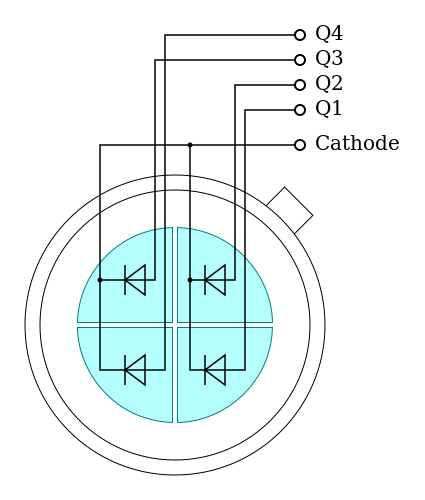
\includegraphics[width=2.5in]{img/Wikipedia/QuadrantenFotodiode.jpg}
	\caption{Quadrantenfotodiode. Quelle: Wikipedia \cite{web:quadrantendiode}}
	\label{fig:quadrantendiode}
\end{figure}

Um nun die Lage eines Laserpunktes bestimmen zu können, werden mehrere Fotodioden benötigt.
Dazu gibt es verschiedene Möglichkeiten diese Fotodioden anzuordnen.
Die bekannteste Variante ist die Quadrantendiode.
Dabei werden vier Fotodioden mit einem kleinen Abstand zwischen den Sensorflächen nebeneinander positioniert.
Die 
In Abbildung~\ref{fig:quadrantendiode} ist eine Quadrantendiode schematisch dargestellt.
Diese können fertig in einem Gehäuse verbaut gekauft werden.
Auch Anordnungen mit mehr als vier Dioden sind erhältlich, sogenannte sedimentierte Fotodioden.

Bei dieser Arbeit werden vier einzelne BPW34 Dioden verwendet.
Für die Schaltung dieses Prototypen kommt eine gemeinsame Anode zum Einsatz, da damit ein OPV mit einer einseitigen Versorgung ausreicht und keine Vorspannung eingestellt werden muss.

\subsection{Auswertung}
\label{chap:elektronik:auswertung}
Um mit der bereits vorgestellten Hardware zu detektieren, wie viel von dem Laserlicht auf die Fläche der Fotodiode fällt, ist ein Algorithmus zur Auswertung notwendig.
Zur Vereinfachung wird angenommen, dass die Ausgangsspannung linear proportional zu dem einfallenden Lichtstrom ist.
Dies ist in der ersten Näherung, wie wir gezeigt haben, auch erfüllt.
Dadurch kann die gemessene Intensität bei eingeschaltetem Laserstrahl von der bei ausgeschaltetem Laserstrahl subtrahiert werden.
Dabei ist allerdings wichtig, dass sich mögliche Störungen langsamer ändern, als die zeitlich Entfernung der Messpunkte.
Da nach dem Einschalten des Lasers, das Ausgangssignal nicht sofort auf den Endwert springt, müssen die in Kapitel~\ref{chap:elektronik:transienteVorgaenge} vermessenen Einschaltvorgänge abgewartet werden.


\subsection{Verbesserte Verfahren}
Eine Verbesserung zu dem bereits vorgestellten Verfahren zur Auswertung der Ausrichtung eines Laserstrahls wäre, den Laserstrahl zu modulieren.
Anstatt nur die auftreffende Intensität mit der Dunkelintensität zu vergleichen, wird ein sinusartiger Lichtstrom erzeugt.
Im Empfänger wird nun mit einem phasenselektiven Synchrongleichrichter (PSSG) oder einem phasenunabhängigen Synchrondemodulator (PUSD) das Signal auf einen bestimmten Frequenzbereich überprüft.
Beide Verfahren stellen schmalbandige Bandpassfilter dar.
Damit lassen sich alle Störungen, welche nicht in der Messfrequenz oder deren Oberschwingungen moduliert sind, unterdrücken.~\cite[210]{book:elektrischeMesstechnik}.

Dazu ist es allerdings notwendig, den Laser auf einem Arbeitspunkt zu modulieren, was mit einer steuerbare Stromquelle realisiert werden kann.
Diese wird mit einem Frequenzgenerator gespeist.
Der Frequenzgenerator ist zum Beispiel durch den DAC des Microcontrollers realisierbar.
Neben dem schaltungstechnisch erhöhten Aufwand wird eine zusätzliche Software auf dem Mikrocontrollers benötigt.
Der wichtigste Nachteil ist allerdings die erhöhte Rechenzeit.
Diese wird benötigt, um das Ausgangssignal zu generieren und eine ausreichend hohe Abtastrate zu erreichen.
Aufgrund der beschränkten Rechenleistung auf dem Mikrocontroller kamen diese Verfahren nicht zum Einsatz.

\chapter{Software}
\label{chap:software}
Dieses Kapitel gibt einen detaillierten Einblick in die Software des Prototypen.


\section{Controller}
\begin{figure}[!h] \centering
	\begin{tikzpicture}[
every node/.style={draw, minimum size=1cm, thick, fill=white, rounded corners},
sam/.style={circle, minimum size=2cm, fill=blue!50},
stm/.style={circle, minimum size=2cm, fill=green!50},
sen/.style={fill=red!50}
]
\node[sam] at (6,0) (sam) {SAM};
\node[stm] at (11,0) (stm) {STM};
\node at (12,3.8) (tln) {Laborteilnehmer};
\node[sen] at (0,3) (li) {Lichtschranken};
\node[sen] at (0,1.5) (ro) {Rotationsencoder};
\node[sen] at (0,0) (fo) {Fotodioden};
\node[sen] at (0,-1.5) (an) {Antriebsmotor};
\node[sen] at (0,-3) (sp) {Spiegelablenkeinheit};

\draw[<->,line width=4pt] (sam) -- (stm);
\draw[<-,line width=2pt] (sam) -- (li.east);
\draw[<-,line width=2pt] (sam) -- (ro.east);
\draw[<-,line width=2pt] (sam) -- (fo.east);
\draw[->,line width=2pt] (sam) -- (an.east);
\draw[->,line width=2pt] (sam) -- (sp.east);
\draw[->,line width=1pt,dashed,double] (tln) -- (stm);

\draw (-2,-4) -- (-2,4) -- (8.5,4) -- (8.5,-4) -- (-2,-4);
\node at (7.8,3.8) (prot) {Prototyp};


\end{tikzpicture}

	\caption{Zusammenspiel der Komponenten}
	\label{fig:samStmSensorsAktuators}
\end{figure}

Bei diesem Prototypen existieren zwei verschiedene Controller, auf denen Software ausgeführt wird.

Der erste ist ein SAM3X8E von Atmel mit einer 32-Bit ARM Cortex-M3 Architektur.
Dieser ist auf dem Entwicklungsboard mit dem Namen "`Arduino Due"' verbaut.
Dieser Controller stellt für die Speicherung des Codes 512~KByte Flash und für Variablen 96~KByte SRAM zur Verfügung.
Auf diesem soll die Verwaltung der Hardware ablaufen.
Die Taktrate beträgt bei diesem Controller 84~MHz.

Der zweite Controller ist ein Entwicklungsboard von ST mit den Namen "`NUCLEO-F334R8"'.
Der verbaute Mikrocontroller ist ein STM32F334R8 mit einer 32-Bit ARM Cortex-M4 Architektur.
Der wesentliche Unterschied zwischen einer M3- und einer M4-Architektur liegt dabei in der zusätzlichen Gleitkommaeinheit (FPU).
Eine FPU reduziert die Dauer von Operationen mit Gleitkommazahlen erheblich.
Als Speicher stehen bei dem STM Controller 64~Kbyte Flash und 12~KByte SRAM zur Verfügung.
Die Taktfrequenz liegt bei 72~MHz.
Dieser Controller ist nur mit dem SAM3X8E verbunden und wird verwendet um den ausführbaren Code der Studierenden abzuarbeiten.
Dabei soll ein Teil der Regelung von den Studenten auf dem STM32 implementiert werden.

Der Vergleich der Controller zeigt, dass der STM32 nur eine geringfügig langsamere Taktfrequenz aufweist, dafür aber eine FPU besitzt, welche einen erheblichen Geschwindigkeitsvorteil bringt.
Der STM32 weist zusätzlich noch deutlich weniger Speicher auf, dies ist jedoch für die vorgesehene Aufgabe keine Einschränkung.
Zusammenfassend kann behauptet werden, wenn die Regelung neben den zusätzlichen Aufgaben auf dem SAM3x8E lauffähig ist, sollte die Implementierung auf dem STM32 auch kein Problem darstellen.

Um die Zusammenhänge der Komponenten deutlich zu machen, wurden die Controller und ihre Verknüpfungen in Abbildung~\ref{fig:samStmSensorsAktuators} grafisch dargestellt.
Der SAM wird als Controller zur Verwaltung der Hardware und als Schnittstelle zu den Studenten verwendet.
Der STM32 wird von den Studenten verwendet und ist nur mit dem SAM verbunden.
Im Folgenden wird vor allem der Code für den SAM erläutert.
Dieser enthält neben der Verwaltung der Hardware auch eine Musterlösung und somit den Teil, welcher im Labor auf den zweiten Controller ausgeführt wird.
Dadurch ist die gesamte Logik, zumindest für diesen Controller, implementiert.
Somit werden Ausschnitte aus dem Code in der für den SAM Controller üblichen Notation dargestellt.
Diese Notation umfasst die gebräuchlichen Typen und Befehle, welche für Arduino beziehungsweise für AVR Mikrocontroller üblich sind.
Dazu zählen auch die Integer-Typen, wie $uint16\_t$, welche in der avr-libc definiert sind.
In dieser Form sind sie auf einem STM32 standardmäßig nicht definiert.


\section{Schrittmotoren}

\subsection{Ablauf}
\label{chap:software:schrittmotoren:ablauf}
Für die Schrittmotoren wird in diesem Prototypen ein Halbschrittbetrieb verwendet.
Eine noch feinere Unterteilung ist, wie in Kapitel~\ref{chap:elektronik:mikroschrittbetrieb} erwähnt, nur begrenzt sinnvoll.
Wie bereits erläutert, können die Schrittmotoren als FSM dargestellt und behandelt werden.
Die FSM für den Halbschrittbetrieb ist in Abbildung~\ref{fig:fsmStepperHalbschritt} dargestellt.

Eine elegante Variante dies zu implementieren ist mittels eines Arrays.
Dazu wird zuerst die FSM als Array dargestellt.

\begin{minipage}{\textwidth}
\begin{lstlisting}
const uint8_t fsm[stateCnt][pinCnt] = {
	{ 1,0, 0,0 },
	{ 1,0, 1,0 },
	{ 0,0, 1,0 },
	{ 0,1, 1,0 },
	{ 0,1, 0,0 },
	{ 0,1, 0,1 },
	{ 0,0, 0,1 },
	{ 1,0, 0,1 }
};
\end{lstlisting}
\end{minipage}


Dabei stellen die beiden Pärchen des Arrays je eine Spule des Motors dar.
Vereinfacht erklärt symbolisiert eine Zahl die normierte Spannung an einem Anschluss der Spule.
Somit steht 1,0 für einen Strom in Bezugsrichtung, 0,1 für einen Strom gegen die Bezugsrichtung und 0,0 oder 1,1 für eine stromfreie Spule.
1,1 sollte jedoch nicht verwendet werden, da dies bei unipolar beschalteten Motoren zu hohen Verlusten führt.

Nun muss von einer Timer-Interrupt-Routine die aktuelle Schrittposition auf die Ausgänge des Mikrocontrollers übernommen werden.
Die Timer-Interrupt-Routine wird so eingestellt, dass sie periodisch mit der maximal erlaubten Schrittgeschwindigkeit aufgerufen wird.
Dies kann mit folgendem Code erreicht werden:

\begin{minipage}{\textwidth}
\begin{lstlisting}
int8_t state = position % stateCnt;
for (uint8_t i = 0; i < pinCnt; i++) {
	digitalWrite(pins[i], fsm[state][i]);
}
\end{lstlisting}
\end{minipage}

Dadurch ergibt sich eine asynchrone Ansteuerung der Schrittmotoren, welche unabhängig von der Geschwindigkeit des Hauptprogramms, die Motoren im richtigen Zeitpunkt ansteuert.
Dies ist deshalb besonders wichtig, da eine zu schnelle oder unregelmäßige Ansteuerung einen Schrittverlust bedeuten kann.

Vollständigkeitshalber sei hier noch erwähnt, dass der Code für einen Mikroschrittbetrieb zwar als FSM darstellbar ist, dies aber nicht zweckmäßig ist.
Eleganter ist es, mit Sinus und Kosinus zu arbeiten.
Da in diesem Fall der Mikroschrittbetrieb ohnehin nicht benötigt wird und die Berechnung von Gleitkommazahlen ohne FPU zeitaufwendig ist, wird bei dem Prototypen diese Methode nicht verwendet.

\subsection{Timing}

\begin{figure} \centering
	\includegraphics[width=0.49\textwidth]{img/PicturesPlots/Timing/StepperLaserPositioner/COPY/CONVERT/SCRN0154_Cutted.jpg}
	\caption{Dauer der Interrupts für Schrittmotoren.}
	\label{fig:interruptStepper}
\end{figure}

Für den Code, welcher in Interrupts ausgeführt wird, ist es von besonderer Bedeutung eine schnelle Verarbeitung zu erzielen.
Wenn in einem Interrupt viel Zeit benötigt wird, können dadurch andere Interrupts am Ausführen gehindert werden.
Dies ist unter allen Umständen zu vermeiden.

Die Frequenz, mit welcher der Interrupt aufgerufen wird, ist fest vorgegeben durch die Schrittgeschwindigkeit.
Der einzige Weg, den Tastgrad der Ausführungszeiten zu variieren ist somit die Rechenzeit.
Das bedeutet, dass die benötigte Rechenzeit kurz genug sein muss, um den restlichen Code nicht zu beeinflussen.

Um diese Anforderung zu überprüfen, sind in Abbildung~\ref{fig:interruptStepper} die Zeiten aufgenommen, in denen die Interrupt-Routine aktiv war.
Dabei ist der gemessene Wert auf 3,3~V wenn der Interrupt aktiv ist und 0~V wenn er nicht aktiv ist.
Der gemessene Tastgrad beträgt 1,6~\%.
Das bedeutet, dass der Interrupt nur 1,6~\% der gesamten Rechenzeit in Anspruch nimmt.
Dieser Wert ist gut vertretbar und es kann angenommen werden, dass der restliche Code unbeeinflusst abgearbeitet werden kann.



\section{Quadratur Encoder}	
Die Implementierung des Quadratur Encoders funktioniert ähnlich wie die Implementierung der Schrittmotoren.
Auch hier muss der bereits in Kapitel~\ref{chap:aufbau:aufbauInkrementalgeberFSM} betrachtete Automat implementiert werden.
Dieser kann wieder in einem Array dargestellt werden.
Hier werden jedoch nicht die Zustände als Werte der Felder verwendet, sondern die Schrittweite.
Die Indizes des Arrays stellen dabei die Zustände dar.

\begin{minipage}{\textwidth}
\begin{lstlisting}
const int8_t encoderFsm[4][4] = {
	{ 0, 1,-1, 0},
	{-1, 0, 0, 1},
	{ 1, 0, 0,-1},
	{ 0,-1, 1, 0}
};
\end{lstlisting}
\end{minipage}

Dabei hat die erste Ziffer des Zustandes die Wertigkeit 2 und die zweite Ziffer die Wertigkeit 1.
Die Zustandsnamen stellen sozusagen den Binärcode der Indizes dar.
Wird nun von dem Zustand 10 auf den Zustand 11 gewechselt, werden die Indizes 2 und 3 abgefragt und das Ergebnis ist die Schrittweite -1.

Eine wichtige Eigenschaft dieser Matrix ist, dass sie schiefsymmetrisch ist.
Das bedeutet, dass die transponierte Matrix negativ ist.
Somit liefert eine Umkehrung der Reihenfolge der Zustände ein negiertes Ergebnis.
Ein ungültiger Übergang, so wie Übergänge von einem Zustand auf sich selbst, liefert in dieser Variante 0.
Als Beispiel kann der Übergang von 01 auf 10 mit den Indizes 1 und 2 betrachtet werden.

Da jedoch Eingangsdaten und nicht Ausgangsdaten behandelt werden, funktioniert hier die Implementierung anders als die Implementierung des Schrittmotors in Kapitel~\ref{chap:software:schrittmotoren:ablauf}.
Zuerst werden die Eingangsdaten benötigt, welche mit $ina$ und $inb$ gekennzeichnet sind.
Zusätzlich ist auch der letzte Zustand von Bedeutung.
Auch dieser wird mit den zugehörigen Eingangsdaten dargestellt, welche mit $lasta$ und $lastb$ benannt sind.
Der nötige Code, um die Position zu berechnen, kann folgendermaßen geschrieben werden.

\begin{minipage}{\textwidth}
\begin{lstlisting}
pos += encoderFsm[(ina << 1) + inb][(lasta << 1) + lastb];
\end{lstlisting}
\end{minipage}

Die Erkennung der großen Marke ist mit den nun berechneten Werten trivial.
Wie in Kapitel~\ref{chap:aufbau:bigMark} bereits erläutert wurde, müssen dazu nur einzelne Schritte detektiert werden, welche ein anderes Vorzeichen aufweisen.
Auch eine Fehlerdetektion ist möglich, wenn in der Matrix spezielle Werte für einen Fehler eingetragen werden.
Ein Fehler entsteht, wenn ein Interrupt am Ausführen gehindert wird.
Dies passiert bei einer zu hohen Drehgeschwindigkeit.
Der hier präsentierte Code wird im optimalen Fall direkt von der Interrupt-Service-Routine (ISR) aufgerufen, welche für die verwendeten Eingangs-Pins zuständig und auf Pegelwechsel programmiert ist.


\section{Auswertung der Fotodioden}

\subsection{Ablauf}

Genau wie bei Schrittmotoren, ist es auch bei der Auswertung der Fotodioden sinnvoll, Interrupts zu verwenden.
Für diesen Prototypen wurde die in Kapitel~\ref{chap:elektronik:auswertung} erläuterte Methodik verwendet.

% Beschreibung der Messung
Das Messen findet in zwei verschiedenen Methoden statt.
Bei der ersten wird zuerst der Wert ermittelt, welchen die Fotodioden bei ausgeschalteten Laser zurückgeben.
Dieser Wert kann nun aufgrund der Linearität in der zweiten Methode dazu verwendet werden, langsame Störungen, wie das Tageslicht, durch Subtraktion zu eliminieren.

Diese beiden Methoden müssen abwechselnd mit Pausen dazwischen ausgeführt werden.
Am besten wird dazu ein Interrupt verwendet.
Dazu muss die Periodendauer des Interrupts bei jeder Abarbeitung umgeschaltet werden.
Die Zeiten werden im folgenden als Messzeit und Wartezeit bezeichnet
Die Messzeit ist jene, welche zwischen den beiden Methoden verstreicht.
Die Wartezeit ist die Zeit, welche zwischen der zweiten Methode und der ersten der nächsten Messung verstreicht.


\subsection{Timing}
% Tastgrad von Codeausführung
Da auch bei den Interrupts für die Fotodioden nicht zu viel Zeit verschwendet werden darf, ist besonders die Einstellung der Messfrequenz wichtig.
Bei den Schrittmotoren war die Messfrequenz gegeben, anders ist dies bei der Auswertung der Fotodioden.
Hier kann die Ausführungszeit für jede der beiden Unterfunktionen als konstant angenommen werden.
Um nun den Tastgrad auf einen vertretbaren Wert zu bringen, darf die Summe von Messzeit und Wartezeit zwischen den Messungen nicht zu niedrig liegen.
Somit muss die Messfrequenz so gewählt werden, dass ein ungestörter Programmablauf der anderen Programmteile gewährleistet werden kann.
Die Messfrequenz muss aber ausreichend hoch sein, um die Regelung nicht negativ zu beeinflussen.
Für diesen Prototypen wurde eine Messfrequenz von 200~Hz empirisch ermittelt.

% Mindestzeitdauern
Der einzige Parameter, welcher nach den bisherigen Festlegungen noch gewählt werden kann, ist die Aufteilung in Messzeit und Wartezeit.
Die Zeitdauern, welche für diese Wartezeiten mindestens eingehalten werden müssen, wurden bereits im Kapitel~\ref{chap:elektronik:transienteVorgaenge} ausgemessen.
Um eine gültige Messung zu gewährleisten, dürfen diese Zeiten auf keinen Fall unterschritten werden.

% Wahrgenommene Intensität
Solange die notwendigen Mindestzeiten eingehalten werden, verändert sich dadurch auch die Qualität der Messung nicht.
Das Verhältnis dieser Werte gibt jedoch die, von menschliche Auge wahrgenommene, Helligkeit des Laserpunktes an.
Ist die Messzeit auf den minimal erlaubten Wert eingestellt, ist der Laserpunkt unter Tageslicht kaum mehr wahrnehmbar.
Bei einer minimalen Wartezeit ergibt sich die maximale Helligkeit des Lasers.
Somit kann als Nebeneffekt dieser Regelung die gewünschte Helligkeit eingestellt werden.
Das Timing der Interrupts ist auch in diesem Fall wieder von besonderem Interesse und wird zur Überprüfung in Abbildung~\ref{fig:interruptFotodioden} dargestellt.
Der Tastgrad ist mit 8,41~\% höher als bei den Schrittmotoren aber immer noch vertretbar.
In dieser Abbildung ist auch ersichtlich, dass die Methode mit unterschiedlichen Wartezeiten aufgerufen wird.
Für diese Aufnahme wurde der Laser auf eine geringe Leuchtkraft eingestellt.
Zwischen zwei nahen Peaks ist also der Zeitraum in denen der Laser leuchtet.

\begin{figure} \centering
	\includegraphics[width=0.49\textwidth]{img/PicturesPlots/Timing/DiodesLaser/COPY/CONVERT/SCRN0160_Cutted.jpg}
	\caption{Timing der Interrupts für die Auswertung der Fotodioden.}
	\label{fig:interruptFotodioden}
\end{figure}


\section{Implementierung einer Regelung}

\subsection{Charakteristik einer Fotodiode}

\begin{figure} \centering
	\input{img/tikz/FotodiodesMeshPlotSingle}
	\caption{Ausgabewerte einer Fotodiode mit und ohne Störeinflüsse, welche im normalen Betrieb auftreten.}
	\label{img:FotodiodesSingle}
\end{figure}

Eine wichtige Grundlage beim Aufbau einer Regelung sind die zur Verfügung stehenden Informationen.
Um sich ein Bild von den möglichen Eingangsdaten zu machen, wurde mit dem Laserstrahl im Halbschrittbetrieb jeder mögliche Punkt auf den Fotodioden abgetastet.
Die Referenzspannung des ADC hat bei der Messung $3.3~V$ betragen und es wurde mit 10~Bit Auflösung gemessen.
Somit entspricht ein digitaler Wert von 1 einer Spannung von $3,22~mV$

Die Daten einer einzelnen Fotodiode wurden in Abbildung~\ref{img:FotodiodesSingle} dargestellt.
Die Grafik gibt dabei detailliert die Ausgangswerte, in Abhängigkeit zu der Schrittposition der beiden Schrittmotoren, an.
Um dabei die Übersichtlichkeit zu erhalten, wurden nur Datenpunkte angegeben, welche einen Wert von mindestens 5 aufweisen, dies entspricht $16,1~mV$.

Eine wichtige Anmerkung ist, dass die rechte Grafik auf einer Messung unter optimalen Bedingungen basiert.
Dabei wurde versucht die Fremdlichtintensität auf ein Minimum zu reduzieren.
Weiteres wurde für einen Aufnahmepunkt über 100 Messungen gemittelt.
Um eine Vorstellung davon zu bekommen, wie diese Einflüsse die Messung beeinflussen können, wurde zum Vergleich das linke Bild unter normalen Bedingungen aufgenommen.
Dabei ist deutlich sichtbar, dass die Werte gewissen Schwankungen unterliegen, die Qualität jedoch ausreichend ist, um damit eine Regelung zu implementieren.


\subsection{Charakteristik aller Fotodioden}

\begin{figure} \centering
	\begin{tikzpicture}[scale=1]
\begin{axis}[surf, z buffer=sort, opacity=0.5, restrict expr to domain={z >= 5}{1:1},xlabel=x,ylabel=y]
\addplot3 [color=red, opacity=1] table[x index=0, y index=1, z index=2, col sep=tab] {img/DiodePositionPlot/DiodePositionPlot04.txt};
\addplot3 [color=blue] table[x index=0, y index=1, z index=3, col sep=tab] {img/DiodePositionPlot/DiodePositionPlot04.txt};
\addplot3 [color=green] table[x index=0, y index=1, z index=4, col sep=tab] {img/DiodePositionPlot/DiodePositionPlot04.txt};
\addplot3 [color=orange, opacity=0.4] table[x index=0, y index=1, z index=5, col sep=tab] {img/DiodePositionPlot/DiodePositionPlot04.txt};
\end{axis}
\end{tikzpicture}
	\caption{Ausgabewerte der Fotodioden in einer gemeinsamen Grafik.}
	\label{img:FotodiodesBig}
\end{figure}

Abbildung~\ref{img:FotodiodesSingle} zeigt neben den bereits diskutierten Eigenschaften auch, dass die Fotodiode bei direkter Bestrahlung sättigt.
Dies ist für eine Regelung durchaus ein Problem und könnte behoben werden, indem der, in Kapitel~\ref{chap:elektronik:tia} besprochene Widerstand, durch einen Kleineren ersetzt wird.
Dadurch verringert sich jedoch auch die Empfindlichkeit am Rand des Messbereiches.

Wenn nun alle vier Fotodioden in ein Bild eingearbeitet werden, sieht man, dass sich die Sättigungsbereiche der Dioden kaum überlappen.
Dies wird in Abbildung~\ref{img:FotodiodesBig} dargestellt.
Selbst wenn man sich nun auf einen Punkt befindet, bei welchem zwei Dioden sättigen, so befindet man sich bereits im Messbereich der anderen beiden Dioden.
Dadurch kann im gemeinsamen Messbereich der Dioden, an den meisten Positionen der Standort bestimmt werden.


\subsection{Entwurf eines Dreipunktreglers}

%Anmerkungen zu Grafiken
Mit den bereits diskutierten Werten werden nun zwei Regler entworfen.
Ein Regler ist zuständig für den Schrittmotor, welcher den Laser horizontal ablenkt, der andere regelt die vertikale Ablenkung.
Um die Diagramme vergleichbar zu machen, zeigen sie in diesem Abschnitt immer den Regler, welcher die lange Seite der Dioden regelt.
Diese Achse wird als x Achse bezeichnen.

%Erklärung zweier Regler
Bei dem Entwurf des Reglers könnte im Folgenden berücksichtigt werden, dass die Fotodioden rechteckig sind.
Würde diese Information jedoch die Regelparameter mitbestimmen, so müsste im folgenden für jede Achse ein Regler mit verschiedenen Parametern verwendet werden.
Das soll hier für die erste Betrachtung jedoch vermieden werden.
Da nun beide Regler äquivalent zueinander sind, ist es ausreichend einen zu entwerfen.

%Einfache Verknüpfung der Daten
Das Ergebnis dieses Entwurfes soll eine Entscheidungsstrategie sein, welche entscheidet, ob der Motor in eine Bezugsrichtung drehen, gegen die Bezugsrichtung drehen oder still stehen soll.
Dafür gibt es verschiedene Strategien die gemessenen Rohdaten aufzubereiten.
So könnte zuerst die Position des Laserpunktes ermittelt werden, um mit dieser Information die Regelung durchzuführen.
Da die Position aber nichtlinear von den Eingangsdaten abhängig ist, ist es einfacher, direkt mit den Eingangsdaten der Dioden zu arbeiten.

\begin{figure} \centering
	\begin{comment}
\begin{tikzpicture}[scale=0.92]
\begin{axis}[xlabel=x,ylabel=y]
\addplot3 [surf, mesh/ordering=y varies, restrict expr to domain={z <= -4 || z >= 4 || (x > 15 && x < 25 && y > 11 && y < 28)}{1:1}] table[x index=0, y index=1, z expr={(\thisrowno{2}-\thisrowno{3})+(\thisrowno{4}-\thisrowno{5})}, col sep=tab] {img/DiodePositionPlot/DiodePositionPlot03.txt};
\end{axis}
\end{tikzpicture}
\begin{tikzpicture}[scale=0.92]
\begin{axis}[xlabel=x,ylabel=y]
\addplot3 [surf, mesh/ordering=y varies, restrict expr to domain={z <= -100 || z >= 100}{1:1}] table[x index=0, y index=1, z expr={(\thisrowno{2}-\thisrowno{3})+(\thisrowno{4}-\thisrowno{5})}, col sep=tab] {img/DiodePositionPlot/DiodePositionPlot03.txt};
\end{axis}
\end{tikzpicture}
\end{comment}
\begin{tikzpicture}[scale=0.92]
\begin{axis}[xlabel=x,ylabel=y]
\addplot3 [surf, mesh/ordering=y varies, restrict expr to domain={z <= -4 || z >= 4 || (x > 15 && x < 25 && y > 11 && y < 28)}{1:1}] table[x index=0, y index=1, z expr={(\thisrowno{2}-\thisrowno{3})+(\thisrowno{4}-\thisrowno{5})}, col sep=tab] {img/DiodePositionPlot/DiodePositionPlot03.txt};
\end{axis}
\end{tikzpicture}
\begin{tikzpicture}[scale=0.92]
\begin{axis}[xlabel=x,ylabel=y]
\addplot3 [surf, mesh/ordering=y varies, restrict expr to domain={z <= -100 || z >= 100}{1:1}] table[x index=0, y index=1, z expr={(\thisrowno{2}-\thisrowno{3})+(\thisrowno{4}-\thisrowno{5})}, col sep=tab] {img/DiodePositionPlot/DiodePositionPlot03.txt};
\end{axis}
\end{tikzpicture}
	\caption{Dreipunktregler basierend auf addierten Messwerten.}
	\label{img:dreipunktreglerAdd}
\end{figure}

Ein erster Ansatz für die Auswertung der Daten ist, die Werte auf der y Achse zu summieren und auf der x Achse zu subtrahieren.
Diese Verknüpfung der Eingangsdaten ist in Abbildung~\ref{img:dreipunktreglerAdd} im linken Bild dargestellt.
Mit den so gewonnenen Daten kann nun ein Dreipunktregler gespeist werden, welcher mit zwei Schaltschwellen entscheidet, wie der Motor angesteuert werden sollen.
Die dabei entstehende Schaltcharakteristik ist in Abbildung~\ref{img:dreipunktreglerAdd} im rechten Bild dargestellt.
Dabei wurden nur jene Bereiche gezeichnet, welche über oder unter möglichen Schwellwerten liegen.
Anders formuliert sind die Punkte des rechten Bildes die Teilmenge der Punkte des linken Bildes, bei der eine Interaktion des Motors erforderlich ist.

\begin{figure} \centering
	\input{img/tikz/FotodiodesMeshPlotMax}
	\caption{Dreipunktregler basierend auf Maximum Werte.}
	\label{img:dreipunktreglerMax}
\end{figure}

%Max Min Verknüpfung
Eine alternative Verknüpfung ist, die y Achse nicht zu summieren, sondern den Maximalwert zu verwenden.
Dadurch können Überhöhungen, welche beim Übergang von einer Fotodiode auf eine andere entstehen, vermieden werden.
Die Eingangsdaten und der Schaltbereich dieser Variante ist in Abbildung~\ref{img:dreipunktreglerMax} dargestellt.
Dabei sind die Unterschiede zur ersten Variante gut erkennbar.
Diese Unterschiede befinden sich hauptsächlich bei den Grenzbereichen der Fotodioden.


\subsection{Implementierung eines Dreipunktreglers}
Im folgenden wird die Implementierung des bereits besprochenen Dreipunktreglers gezeigt.
Dabei wird die erste Variante erläutert, bei der die Eingangswerte additiv verknüpft werden.

%Abarbeitungszyklus
Es ist wichtig, dass der Regler mit einer konstanten Frequenz periodisch aufgerufen wird.
Um eine konstante Frequenz zu gewährleisten, könnte der Regler mit einem Timer-Interrupt ausgeführt werden.
Da der Regler allerdings viele Gleitkommaoperationen benötigt und deshalb eine lange Verarbeitungszeit benötigt wird, ist dies nicht zu empfehlen.
Stattdessen wird der Regler in der Hauptschleife abgearbeitet und es wird versucht die anderen Aufgaben in Interrupts zu verlagern.
Um dabei eine konstante Abtastfrequenz zu erhalten, wird nach jedem Zyklus solange gewartet, bis der reziproke Wert der Update-Frequenz erreicht ist.

%Erklärung des Reglers
Diese Implementierung beinhaltet drei Teilaufgaben.
Die erste ist das Errechnen und Mitteln des Wertes für den Dreipunktregler.
Zur Mittlung wird ein Infinity Impulse Response (IIR) Tiefpassfilter erster Ordnung verwendet.
Der Vorteil dieses IIR Filter ist seine einfache Implementierung.
Dies kann mit folgendem Code erreicht werden.

\begin{minipage}{\textwidth}
\begin{lstlisting}
horizontal = diodeLU + diodeLD - diodeRU - diodeRD;
vertical = diodeLU + diodeRU - diodeLD - diodeRD;
lowHor = (lowHor*filterParam + horizontal) / (filterParam + 1);
lowVer = (lowVer*filterParam + vertical) / (filterParam + 1);
\end{lstlisting}
\end{minipage}

Eine schnellere und präzisere Reaktion des Reglers kann dadurch erreicht werden, dass der Filter häufiger ausgeführt wird als der Regler.
Dies sorgt für eine genauere Messung und reduziert das Rauschen und sonstige unkorrelierte Messfehler.

Die zweite Teilaufgabe ist die Berücksichtigung der Drehung der Encoderscheibe.
Dazu wird, mit dem vom Drehgeber generierten Winkel, das Koordinatensystem der Fotodioden in das der Spiegelablenkeinheit umgerechnet.
Dies kann, da die Drehung nur um die z Achse verläuft, mit einer Multiplikation mit Sinus und Kosinus erfolgen.

\begin{minipage}{\textwidth}
	\begin{lstlisting}
	double h = cos(encoderAngle);
	double v = sin(encoderAngle);
	\end{lstlisting}
\end{minipage}

Die letzte Aufgabe besteht darin, zu entscheiden ob, eine der Schaltschwellen erreicht wurde.
Wenn dies der Fall ist, kann ein Koordinaten transformierter Schritt ausgeführt werden.

\begin{minipage}{\textwidth}
\begin{lstlisting}
if (lowVer > triggerLevel) {
	stepperPosV += cosV;
	stepperPosH -= sinV;
} else if (lowVer < -triggerLevel) {
	stepperPosV -= cosV;
	stepperPosH += sinV;
}
if (lowHor > triggerLevel) {
	stepperPosH += cosV;
	stepperPosV += sinV;
} else if (lowHor < -triggerLevel) {
	stepperPosH -= cosV;
	stepperPosV -= sinV;
}
\end{lstlisting}
\end{minipage}

Hier ist es auch möglich, nicht nur einen Schritt sondern mehrere zu machen.
Ein Schritt bezeichnet dabei die kleinste verwendete Unterteilung.
Bei dem Prototypen ist dies ein Halbschritt für den Motor.

Dabei sind zwei Punkte zu beachten, damit der Regler gut funktionieren kann.
Zum ersten müssen die Schritte gerundet werden, bevor sie dem Schrittmotor als Eingangssignal gegeben werden.
Dies ist nachvollziehbar, da immer nur ein vollständiger Schritt ausgeführt werden kann, wenn nicht eine weitere Schrittteilung vorgenommen wird.

Der zweite Punkt ist, dass nicht mehr Schritte von der Regelung generiert werden dürfen, als der Motor wirklich umsetzen kann.
Dies ist für die Regelung von großer Bedeutung, da diese dadurch instabil werden kann, wenn die Motoren asynchron angesteuert werden.
Hat der Regler eine höhere Abtastrate hat als die Schrittfrequenz der Motoren, dann generiert der Regler Schritte ohne dass die Motoren die letzte Position überhaupt erreicht haben.
Erreicht der Motor danach die Soll-Position, generiert der Regler keinen Schritt mehr, die Motoren haben aber noch nicht abgearbeitete Schritte.
Dies führt zu einem Überschwingen oder zu einem instabilen Regler.

\chapter{Zusammenfassung}
\label{chap:zusammenfassung}

In dieser Arbeit wurde ein Prototyp vorgestellt, der in Zukunft in der Lehrveranstaltung "`Mikrocomputer Labor"' verwendet werden soll.
Die Aufgaben, welche von den Studierenden gelöst werden müssen, sind Teilaufgaben der Regelung einer Spiegelablenkeinheit auf eine Scheibe mit einem Detektor.

Bei Arbeiten, welche einen repräsentativen Charakter haben, gibt es neben den technischen Eigenschaften auch gewisse Voraussetzungen, welche das Design der Arbeit betreffen.
Dadurch treten Probleme auf, mit denen normalerweise nicht gerechnet werden können.
Das am Anfang geplante Pendel war technisch gesehen voll funktionsfähig, jedoch war dieses optisch nicht ansprechend.
Unregelmäßige Schwingeigenschaften und eine zu instabile Konstruktionen waren die größte Probleme, weshalb das Pendel durch eine Scheibe ersetzt wurde.

Viele Schwierigkeiten dieser Arbeit sind bei der Erkennung des Lasers gelegen.
Dafür musste nicht nur ein geeignetes Verfahren gesucht werden, sondern auch die Aufbereitung der so gewonnenen Informationen ist ein interessanter Aufgabenbereich.
In diesem Teil der Arbeit gibt es durchaus noch Herausforderungen wie das Implementieren eines PSSG oder eines PUSD.

Eine weiterer interessanter Themenbereich, welcher in dieser Arbeit nur kurz angeschnitten wurde, ist die verwendete Regelung.
Der Übergang von einem Dreipunktregler zu einem Zustandsregler oder anderen Verfahren, würde dabei eine merkbare Verbesserung der Regeleigenschaften versprechen.

%Wichtigsten Ergebnisse / Was soll sich Leser merken?
%Unvorhergesehene Schwierigkeiten / Lösungen
%-Pendel
%Offene Fragen für weiteren Arbeit
%-PSSG / PUSD
%-Verbesserter Regelalgorithmus




%%%%%%%%%%%%%%%%%%%%%%%%%%%%%%%%%%%%%%%%%%%%%%%
% 6.Appendices
%%%%%%%%%%%%%%%%%%%%%%%%%%%%%%%%%%%%%%%%%%%%%%%

% defines epmty pages except pagenumber in the footer
% generagtes the List of Figures (extension: *.lof)
%\listoffigures
% generates the List of Tables (extension: *.lot)
%\listoftables

% generates the List of Examples and adds it to the toc. If you make use of
% the example-environment uncomment the following lines.
%\listof{example}
%{List of Examples
% \protect
% \addcontentsline{toc}{chapter}{List of Examples}
%}
\pagestyle{empty}
\newpage
\pagestyle{fancyplain}

% generates the aux-Files with citations
% \nocite{*}
% this reads the bbl files and makes the bibliography
\newpage
\setlength{\bibsep}{0.0pt}

\renewcommand\bibname{Wissenschaftliche Literatur}
\addcontentsline{toc}{chapter}{Wissenschaftliche Literatur}

\label{lit}
\bibliography{literature}
% the style of bibliography
% start a new page
\bibliographystyle{alphadin}


\addcontentsline{toc}{chapter}{Internet Referenzen}
\def\@newusecounter#1{\@nmbrlisttrue\def\@listctr{#1}}
\let\newusecounter\usecounter

\label{wlit}
\bibliographyweblink{weblinks}
\bibliographystyleweblink{abbrv}
\newpage

\listoffigures


%%%%%%%%%%%%%%%%%%%%%%%%%%%%%%%%%%%%%%%%%%%%%%%
% 7.Official copyright statement
%%%%%%%%%%%%%%%%%%%%%%%%%%%%%%%%%%%%%%%%%%%%%%%


%%%%%%%%%%%%%%%%%%%%%%%%%%%%%%%%%%%%%%%%%%%%%%%%%%%%%%%%%%%%%%%%%%%%%%%
% Official copyright statement for your thesis                        %
%%%%%%%%%%%%%%%%%%%%%%%%%%%%%%%%%%%%%%%%%%%%%%%%%%%%%%%%%%%%%%%%%%%%%%%

\pagestyle{empty}
\newpage
\vspace*{5 cm}
\begin{center}
Erklärung
\end{center}
\vfill
\emph{Hiermit erkläre ich, dass die vorliegende Arbeit ohne unzulässige Hilfe
Dritter und ohne Benutzung anderer als der angegebenen Hilfsmittel angefertigt
wurde. Die aus anderen Quellen oder indirekt übernommenen Daten und Konzepte
sind unter Angabe der Quelle gekennzeichnet.\\\vfill Die Arbeit wurde bisher
weder im In- noch im Ausland in gleicher oder in ähnlicher Form in anderen
Prüfungsverfahren vorgelegt.}
\\\vfill
Wien, am \today\hfill\hrulefill
\vfill
\begin{flushright}
Andreas Gruber\\
\vspace*{5 cm}
\vfill
\end{flushright}
\newpage






\end{document}








